% Options for packages loaded elsewhere
\PassOptionsToPackage{unicode}{hyperref}
\PassOptionsToPackage{hyphens}{url}
\PassOptionsToPackage{dvipsnames,svgnames,x11names}{xcolor}
%
\documentclass[
  letterpaper,
  DIV=11,
  numbers=noendperiod]{scrartcl}

\usepackage{amsmath,amssymb}
\usepackage{lmodern}
\usepackage{iftex}
\ifPDFTeX
  \usepackage[T1]{fontenc}
  \usepackage[utf8]{inputenc}
  \usepackage{textcomp} % provide euro and other symbols
\else % if luatex or xetex
  \usepackage{unicode-math}
  \defaultfontfeatures{Scale=MatchLowercase}
  \defaultfontfeatures[\rmfamily]{Ligatures=TeX,Scale=1}
  \setmainfont[]{Cambria}
\fi
% Use upquote if available, for straight quotes in verbatim environments
\IfFileExists{upquote.sty}{\usepackage{upquote}}{}
\IfFileExists{microtype.sty}{% use microtype if available
  \usepackage[]{microtype}
  \UseMicrotypeSet[protrusion]{basicmath} % disable protrusion for tt fonts
}{}
\makeatletter
\@ifundefined{KOMAClassName}{% if non-KOMA class
  \IfFileExists{parskip.sty}{%
    \usepackage{parskip}
  }{% else
    \setlength{\parindent}{0pt}
    \setlength{\parskip}{6pt plus 2pt minus 1pt}}
}{% if KOMA class
  \KOMAoptions{parskip=half}}
\makeatother
\usepackage{xcolor}
\setlength{\emergencystretch}{3em} % prevent overfull lines
\setcounter{secnumdepth}{-\maxdimen} % remove section numbering
% Make \paragraph and \subparagraph free-standing
\ifx\paragraph\undefined\else
  \let\oldparagraph\paragraph
  \renewcommand{\paragraph}[1]{\oldparagraph{#1}\mbox{}}
\fi
\ifx\subparagraph\undefined\else
  \let\oldsubparagraph\subparagraph
  \renewcommand{\subparagraph}[1]{\oldsubparagraph{#1}\mbox{}}
\fi

\usepackage{color}
\usepackage{fancyvrb}
\newcommand{\VerbBar}{|}
\newcommand{\VERB}{\Verb[commandchars=\\\{\}]}
\DefineVerbatimEnvironment{Highlighting}{Verbatim}{commandchars=\\\{\}}
% Add ',fontsize=\small' for more characters per line
\usepackage{framed}
\definecolor{shadecolor}{RGB}{241,243,245}
\newenvironment{Shaded}{\begin{snugshade}}{\end{snugshade}}
\newcommand{\AlertTok}[1]{\textcolor[rgb]{0.68,0.00,0.00}{#1}}
\newcommand{\AnnotationTok}[1]{\textcolor[rgb]{0.37,0.37,0.37}{#1}}
\newcommand{\AttributeTok}[1]{\textcolor[rgb]{0.40,0.45,0.13}{#1}}
\newcommand{\BaseNTok}[1]{\textcolor[rgb]{0.68,0.00,0.00}{#1}}
\newcommand{\BuiltInTok}[1]{\textcolor[rgb]{0.00,0.23,0.31}{#1}}
\newcommand{\CharTok}[1]{\textcolor[rgb]{0.13,0.47,0.30}{#1}}
\newcommand{\CommentTok}[1]{\textcolor[rgb]{0.37,0.37,0.37}{#1}}
\newcommand{\CommentVarTok}[1]{\textcolor[rgb]{0.37,0.37,0.37}{\textit{#1}}}
\newcommand{\ConstantTok}[1]{\textcolor[rgb]{0.56,0.35,0.01}{#1}}
\newcommand{\ControlFlowTok}[1]{\textcolor[rgb]{0.00,0.23,0.31}{#1}}
\newcommand{\DataTypeTok}[1]{\textcolor[rgb]{0.68,0.00,0.00}{#1}}
\newcommand{\DecValTok}[1]{\textcolor[rgb]{0.68,0.00,0.00}{#1}}
\newcommand{\DocumentationTok}[1]{\textcolor[rgb]{0.37,0.37,0.37}{\textit{#1}}}
\newcommand{\ErrorTok}[1]{\textcolor[rgb]{0.68,0.00,0.00}{#1}}
\newcommand{\ExtensionTok}[1]{\textcolor[rgb]{0.00,0.23,0.31}{#1}}
\newcommand{\FloatTok}[1]{\textcolor[rgb]{0.68,0.00,0.00}{#1}}
\newcommand{\FunctionTok}[1]{\textcolor[rgb]{0.28,0.35,0.67}{#1}}
\newcommand{\ImportTok}[1]{\textcolor[rgb]{0.00,0.46,0.62}{#1}}
\newcommand{\InformationTok}[1]{\textcolor[rgb]{0.37,0.37,0.37}{#1}}
\newcommand{\KeywordTok}[1]{\textcolor[rgb]{0.00,0.23,0.31}{#1}}
\newcommand{\NormalTok}[1]{\textcolor[rgb]{0.00,0.23,0.31}{#1}}
\newcommand{\OperatorTok}[1]{\textcolor[rgb]{0.37,0.37,0.37}{#1}}
\newcommand{\OtherTok}[1]{\textcolor[rgb]{0.00,0.23,0.31}{#1}}
\newcommand{\PreprocessorTok}[1]{\textcolor[rgb]{0.68,0.00,0.00}{#1}}
\newcommand{\RegionMarkerTok}[1]{\textcolor[rgb]{0.00,0.23,0.31}{#1}}
\newcommand{\SpecialCharTok}[1]{\textcolor[rgb]{0.37,0.37,0.37}{#1}}
\newcommand{\SpecialStringTok}[1]{\textcolor[rgb]{0.13,0.47,0.30}{#1}}
\newcommand{\StringTok}[1]{\textcolor[rgb]{0.13,0.47,0.30}{#1}}
\newcommand{\VariableTok}[1]{\textcolor[rgb]{0.07,0.07,0.07}{#1}}
\newcommand{\VerbatimStringTok}[1]{\textcolor[rgb]{0.13,0.47,0.30}{#1}}
\newcommand{\WarningTok}[1]{\textcolor[rgb]{0.37,0.37,0.37}{\textit{#1}}}

\providecommand{\tightlist}{%
  \setlength{\itemsep}{0pt}\setlength{\parskip}{0pt}}\usepackage{longtable,booktabs,array}
\usepackage{calc} % for calculating minipage widths
% Correct order of tables after \paragraph or \subparagraph
\usepackage{etoolbox}
\makeatletter
\patchcmd\longtable{\par}{\if@noskipsec\mbox{}\fi\par}{}{}
\makeatother
% Allow footnotes in longtable head/foot
\IfFileExists{footnotehyper.sty}{\usepackage{footnotehyper}}{\usepackage{footnote}}
\makesavenoteenv{longtable}
\usepackage{graphicx}
\makeatletter
\def\maxwidth{\ifdim\Gin@nat@width>\linewidth\linewidth\else\Gin@nat@width\fi}
\def\maxheight{\ifdim\Gin@nat@height>\textheight\textheight\else\Gin@nat@height\fi}
\makeatother
% Scale images if necessary, so that they will not overflow the page
% margins by default, and it is still possible to overwrite the defaults
% using explicit options in \includegraphics[width, height, ...]{}
\setkeys{Gin}{width=\maxwidth,height=\maxheight,keepaspectratio}
% Set default figure placement to htbp
\makeatletter
\def\fps@figure{htbp}
\makeatother

\usepackage{booktabs}
\usepackage{longtable}
\usepackage{array}
\usepackage{multirow}
\usepackage{wrapfig}
\usepackage{float}
\usepackage{colortbl}
\usepackage{pdflscape}
\usepackage{tabu}
\usepackage{threeparttable}
\usepackage{threeparttablex}
\usepackage[normalem]{ulem}
\usepackage{makecell}
\usepackage{xcolor}
\usepackage{siunitx}

  \newcolumntype{d}{S[
    input-open-uncertainty=,
    input-close-uncertainty=,
    parse-numbers = false,
    table-align-text-pre=false,
    table-align-text-post=false
  ]}
  
\KOMAoption{captions}{tableheading,figureheading}
\makeatletter
\makeatother
\makeatletter
\makeatother
\makeatletter
\@ifpackageloaded{caption}{}{\usepackage{caption}}
\AtBeginDocument{%
\ifdefined\contentsname
  \renewcommand*\contentsname{Table of contents}
\else
  \newcommand\contentsname{Table of contents}
\fi
\ifdefined\listfigurename
  \renewcommand*\listfigurename{List of Figures}
\else
  \newcommand\listfigurename{List of Figures}
\fi
\ifdefined\listtablename
  \renewcommand*\listtablename{List of Tables}
\else
  \newcommand\listtablename{List of Tables}
\fi
\ifdefined\figurename
  \renewcommand*\figurename{Figure}
\else
  \newcommand\figurename{Figure}
\fi
\ifdefined\tablename
  \renewcommand*\tablename{Table}
\else
  \newcommand\tablename{Table}
\fi
}
\@ifpackageloaded{float}{}{\usepackage{float}}
\floatstyle{ruled}
\@ifundefined{c@chapter}{\newfloat{codelisting}{h}{lop}}{\newfloat{codelisting}{h}{lop}[chapter]}
\floatname{codelisting}{Listing}
\newcommand*\listoflistings{\listof{codelisting}{List of Listings}}
\makeatother
\makeatletter
\@ifpackageloaded{caption}{}{\usepackage{caption}}
\@ifpackageloaded{subcaption}{}{\usepackage{subcaption}}
\makeatother
\makeatletter
\@ifpackageloaded{tcolorbox}{}{\usepackage[many]{tcolorbox}}
\makeatother
\makeatletter
\@ifundefined{shadecolor}{\definecolor{shadecolor}{rgb}{.97, .97, .97}}
\makeatother
\makeatletter
\makeatother
\ifLuaTeX
  \usepackage{selnolig}  % disable illegal ligatures
\fi
\IfFileExists{bookmark.sty}{\usepackage{bookmark}}{\usepackage{hyperref}}
\IfFileExists{xurl.sty}{\usepackage{xurl}}{} % add URL line breaks if available
\urlstyle{same} % disable monospaced font for URLs
\hypersetup{
  pdftitle={Problem set 8: The Health Insurance Subsidy Program},
  pdfauthor={Jamie Pantazi Esmond},
  colorlinks=true,
  linkcolor={blue},
  filecolor={Maroon},
  citecolor={Blue},
  urlcolor={Blue},
  pdfcreator={LaTeX via pandoc}}

\title{Problem set 8: The Health Insurance Subsidy Program}
\author{Jamie Pantazi Esmond}
\date{April 15, 2023}

\begin{document}
\maketitle
\ifdefined\Shaded\renewenvironment{Shaded}{\begin{tcolorbox}[boxrule=0pt, borderline west={3pt}{0pt}{shadecolor}, breakable, sharp corners, enhanced, frame hidden, interior hidden]}{\end{tcolorbox}}\fi

\renewcommand*\contentsname{Table of contents}
{
\hypersetup{linkcolor=}
\setcounter{tocdepth}{3}
\tableofcontents
}
\listoffigures
\listoftables
\begin{center}\rule{0.5\linewidth}{0.5pt}\end{center}

\newpage

\begin{Shaded}
\begin{Highlighting}[numbers=left,,]
\FunctionTok{library}\NormalTok{(tidyverse)     }\CommentTok{\# For ggplot, mutate(), filter(), and friends}
\FunctionTok{library}\NormalTok{(broom)         }\CommentTok{\# For converting models to data frames}
\FunctionTok{library}\NormalTok{(estimatr)      }\CommentTok{\# For lm\_robust() and iv\_robust()}
\FunctionTok{library}\NormalTok{(modelsummary)  }\CommentTok{\# For showing side{-}by{-}side regression tables}
\FunctionTok{library}\NormalTok{(MatchIt)       }\CommentTok{\# For matching}
\FunctionTok{library}\NormalTok{(rdrobust)      }\CommentTok{\# For nonparametric RD}
\FunctionTok{library}\NormalTok{(rddensity)     }\CommentTok{\# For nonparametric RD density tests}
\FunctionTok{library}\NormalTok{(haven)         }\CommentTok{\# For reading Stata files}
\FunctionTok{library}\NormalTok{(kableExtra)  }

\NormalTok{knitr}\SpecialCharTok{::}\NormalTok{opts\_chunk}\SpecialCharTok{$}\FunctionTok{set}\NormalTok{(}\AttributeTok{message =} \ConstantTok{FALSE}\NormalTok{, }\AttributeTok{warning =} \ConstantTok{FALSE}\NormalTok{)}

\FunctionTok{set.seed}\NormalTok{(}\DecValTok{80085}\NormalTok{)  }\CommentTok{\# Make any random stuff be the same every time you run this}

\CommentTok{\# Round everything to 3 digits by default}
\FunctionTok{options}\NormalTok{(}\StringTok{"digits"} \OtherTok{=} \DecValTok{3}\NormalTok{)}

\CommentTok{\# Turn off the message that happens when you use group\_by() and summarize()}
\FunctionTok{options}\NormalTok{(}\AttributeTok{dplyr.summarise.inform =} \ConstantTok{FALSE}\NormalTok{)}

\CommentTok{\# Load raw data}
\NormalTok{hisp\_raw }\OtherTok{\textless{}{-}} \FunctionTok{read\_stata}\NormalTok{(}\StringTok{"data/evaluation.dta"}\NormalTok{)}

\CommentTok{\# Make nice clean dataset to use for the rest of the assignment}
\NormalTok{hisp }\OtherTok{\textless{}{-}}\NormalTok{ hisp\_raw }\SpecialCharTok{\%\textgreater{}\%} 
  \CommentTok{\# Having a numeric 0/1 column is sometimes helpful for things that don\textquotesingle{}t like}
  \CommentTok{\# categories, like matchit()}
  \FunctionTok{mutate}\NormalTok{(}\AttributeTok{enrolled\_num =}\NormalTok{ enrolled) }\SpecialCharTok{\%\textgreater{}\%} 
  \CommentTok{\# Convert these 0/1 values to actual categories}
  \FunctionTok{mutate}\NormalTok{(}\AttributeTok{eligible =} \FunctionTok{factor}\NormalTok{(eligible, }\AttributeTok{labels =} \FunctionTok{c}\NormalTok{(}\StringTok{"Not eligible"}\NormalTok{, }\StringTok{"Eligible"}\NormalTok{)),}
         \AttributeTok{enrolled =} \FunctionTok{factor}\NormalTok{(enrolled, }\AttributeTok{labels =} \FunctionTok{c}\NormalTok{(}\StringTok{"Not enrolled"}\NormalTok{, }\StringTok{"Enrolled"}\NormalTok{)),}
         \AttributeTok{round =} \FunctionTok{factor}\NormalTok{(round, }\AttributeTok{labels =} \FunctionTok{c}\NormalTok{(}\StringTok{"Before"}\NormalTok{, }\StringTok{"After"}\NormalTok{)),}
         \AttributeTok{treatment\_locality =} \FunctionTok{factor}\NormalTok{(treatment\_locality, }
                                     \AttributeTok{labels =} \FunctionTok{c}\NormalTok{(}\StringTok{"Control"}\NormalTok{, }\StringTok{"Treatment"}\NormalTok{)),}
         \AttributeTok{promotion\_locality =} \FunctionTok{factor}\NormalTok{(promotion\_locality, }
                                     \AttributeTok{labels =} \FunctionTok{c}\NormalTok{(}\StringTok{"No promotion"}\NormalTok{, }\StringTok{"Promotion"}\NormalTok{))) }\SpecialCharTok{\%\textgreater{}\%} 
  \CommentTok{\# Get rid of this hospital column because (1) we\textquotesingle{}re not using it, and (2) half}
  \CommentTok{\# of the households are missing data, and matchit() complains if any data is}
  \CommentTok{\# missing, even if you\textquotesingle{}re not using it}
  \FunctionTok{select}\NormalTok{(}\SpecialCharTok{{-}}\NormalTok{hospital)}
\end{Highlighting}
\end{Shaded}

The World Bank's \emph{Impact Evaluation in Practice} has used a
hypothetical example of a health insurance program throughout the book.
This Health Insurance Subsidy Program (HISP) provides subsidies for
buying private health insurance to poorer households, with the goal of
lowering personal health expenditures, since people can rely on
insurance coverage instead of paying out-of-pocket. Think of the HISP as
a version of the Affordable Care Act (ACA, commonly known as Obamacare).

The dataset includes a number of important variables you'll use
throughout this assignment:

\begin{longtable}[]{@{}
  >{\raggedright\arraybackslash}p{(\columnwidth - 2\tabcolsep) * \real{0.2471}}
  >{\raggedright\arraybackslash}p{(\columnwidth - 2\tabcolsep) * \real{0.7529}}@{}}
\toprule()
\begin{minipage}[b]{\linewidth}\raggedright
Variable name
\end{minipage} & \begin{minipage}[b]{\linewidth}\raggedright
Description
\end{minipage} \\
\midrule()
\endhead
\texttt{health\_expenditures} & Out of pocket health expenditures (per
person per year) \\
\texttt{eligible} & Household eligible to enroll in HISP \\
\texttt{enrolled} & Household enrolled in HISP \\
\texttt{round} & Indicator for before and after intervention \\
\texttt{treatment\_locality} & Household is located in treatment
community \\
\texttt{poverty\_index} & 1-100 scale of poverty \\
\texttt{promotion\_locality} & Household is located in community that
received random promotion \\
\texttt{enrolled\_rp} & Household enrolled in HISP following random
promotion \\
\bottomrule()
\end{longtable}

It also includes several demographic variables about the households.
\textbf{Each of these are backdoor confounders between health
expenditures participation in the HISP}:

\begin{longtable}[]{@{}
  >{\raggedright\arraybackslash}p{(\columnwidth - 2\tabcolsep) * \real{0.2500}}
  >{\raggedright\arraybackslash}p{(\columnwidth - 2\tabcolsep) * \real{0.7500}}@{}}
\toprule()
\begin{minipage}[b]{\linewidth}\raggedright
Variable name
\end{minipage} & \begin{minipage}[b]{\linewidth}\raggedright
Description
\end{minipage} \\
\midrule()
\endhead
\texttt{age\_hh} & Age of the head of household (years) \\
\texttt{age\_sp} & Age of the spouse (years) \\
\texttt{educ\_hh} & Education of the head of household (years) \\
\texttt{educ\_sp} & Education of the spouse (years) \\
\texttt{female\_hh} & Head of household is a woman (1 = yes) \\
\texttt{indigenous} & Head of household speaks an indigenous language (1
= yes) \\
\texttt{hhsize} & Number of household members \\
\texttt{dirtfloor} & Home has a dirt floor (1 = yes) \\
\texttt{bathroom} & Home has a private bathroom (1 = yes) \\
\texttt{land} & Number of hectares of land owned by household \\
\texttt{hospital\_distance} & Distance to closest hospital (km) \\
\bottomrule()
\end{longtable}

You will use each of the five main econometric approaches for estimating
causal effects to measure the effect of HISP on household health
expenditures. \textbf{Don't worry about conducting in-depth baseline
checks and robustness checks.} For the sake of this assignment, you'll
do the minimum amount of work for each method to determine the causal
effect of the program.

\newpage

\hypertarget{task-1-rcts}{%
\section{Task 1: RCTs}\label{task-1-rcts}}

To measure the effect of HISP accurately, World Bank researchers
randomly assigned different localities (villages, towns, cities,
whatever) to treatment and control groups. Some localities were allowed
to join HISP; others weren't.

Here's what you should do:

\begin{itemize}
\tightlist
\item
  Make a new dataset that only looks at eligible households
  (\texttt{filter(eligible\ ==\ "Eligible")})
\end{itemize}

\begin{Shaded}
\begin{Highlighting}[numbers=left,,]
\NormalTok{eligible }\OtherTok{\textless{}{-}}\NormalTok{ hisp }\SpecialCharTok{\%\textgreater{}\%} 
  \FunctionTok{filter}\NormalTok{(eligible }\SpecialCharTok{==} \StringTok{"Eligible"}\NormalTok{)}
\end{Highlighting}
\end{Shaded}

\begin{itemize}
\tightlist
\item
  Make a new dataset that only looks at eligible households \emph{after}
  the experiment (\texttt{filter(round\ ==\ "After")})
\end{itemize}

\begin{Shaded}
\begin{Highlighting}[numbers=left,,]
\NormalTok{after\_elig }\OtherTok{\textless{}{-}}\NormalTok{ eligible }\SpecialCharTok{\%\textgreater{}\%} 
  \FunctionTok{filter}\NormalTok{(round }\SpecialCharTok{==} \StringTok{"After"}\NormalTok{)}
\end{Highlighting}
\end{Shaded}

\begin{itemize}
\tightlist
\item
  Calculate the average health expenditures in treatment and control
  localities (\texttt{treatment\_locality}) \emph{before} the
  intervention (\texttt{round\ ==\ "Before"}). Were expenditures fairly
  balanced across treatment and control groups before the intervention?
\end{itemize}

\begin{Shaded}
\begin{Highlighting}[numbers=left,,]
\NormalTok{b4 }\OtherTok{\textless{}{-}}\NormalTok{ hisp }\SpecialCharTok{\%\textgreater{}\%} 
  \FunctionTok{filter}\NormalTok{(round }\SpecialCharTok{==} \StringTok{"Before"}\NormalTok{) }\SpecialCharTok{\%\textgreater{}\%} 
  \FunctionTok{group\_by}\NormalTok{(treatment\_locality) }\SpecialCharTok{\%\textgreater{}\%} 
  \FunctionTok{summarise}\NormalTok{(}\AttributeTok{loc\_mean =} \FunctionTok{mean}\NormalTok{(health\_expenditures))}

\NormalTok{b4}
\end{Highlighting}
\end{Shaded}

\begin{verbatim}
# A tibble: 2 x 2
  treatment_locality loc_mean
  <fct>                 <dbl>
1 Control                17.4
2 Treatment              17.0
\end{verbatim}

\begin{itemize}
\item
  \textbf{Yes, the treatment and control groups are fairly balanced
  before the treatment; there was only a 0.372 difference.}
\item
  Calculate the average health expenditures in treatment and control
  localities \emph{after} the intervention (\texttt{round\ ==\ "After"})
\end{itemize}

\begin{Shaded}
\begin{Highlighting}[numbers=left,,]
\NormalTok{after }\OtherTok{\textless{}{-}}\NormalTok{ hisp }\SpecialCharTok{\%\textgreater{}\%} 
  \FunctionTok{filter}\NormalTok{(round }\SpecialCharTok{==} \StringTok{"After"}\NormalTok{) }\SpecialCharTok{\%\textgreater{}\%} 
  \FunctionTok{group\_by}\NormalTok{(treatment\_locality) }\SpecialCharTok{\%\textgreater{}\%} 
  \FunctionTok{summarise}\NormalTok{(}\AttributeTok{loc\_mean =} \FunctionTok{mean}\NormalTok{(health\_expenditures))}

\NormalTok{after}
\end{Highlighting}
\end{Shaded}

\begin{verbatim}
# A tibble: 2 x 2
  treatment_locality loc_mean
  <fct>                 <dbl>
1 Control                20.1
2 Treatment              13.7
\end{verbatim}

\begin{itemize}
\tightlist
\item
  Determine the difference in average health expenditures across
  treatment and control \emph{after} the intervention

  \begin{itemize}
  \tightlist
  \item
    \textbf{After the treatment, the treatment and control groups now
    vary in average health expenditures; the difference is now 6.406, in
    favor of the treatment group.}
  \end{itemize}
\item
  Using data \emph{after} the intervention, use linear regression to
  determine the difference in means and statistical significance of the
  difference (hint: you'll want to use
  \texttt{health\_expenditures\ \textasciitilde{}\ treatment\_locality}).
  Use \texttt{lm\_robust()} from the \textbf{estimatr} package and
  cluster by \texttt{locality\_identifier} if you're feeling
  adventurous.
\end{itemize}

\begin{Shaded}
\begin{Highlighting}[numbers=left,,]
\NormalTok{all\_after }\OtherTok{\textless{}{-}}\NormalTok{ hisp }\SpecialCharTok{\%\textgreater{}\%} 
  \FunctionTok{filter}\NormalTok{(round }\SpecialCharTok{==} \StringTok{"After"}\NormalTok{) }

\NormalTok{he\_after }\OtherTok{\textless{}{-}} \FunctionTok{lm}\NormalTok{(health\_expenditures }\SpecialCharTok{\textasciitilde{}}\NormalTok{ treatment\_locality, }\AttributeTok{data =}\NormalTok{ all\_after)}
\FunctionTok{tidy}\NormalTok{(he\_after)}
\end{Highlighting}
\end{Shaded}

\begin{verbatim}
# A tibble: 2 x 5
  term                        estimate std.error statistic   p.value
  <chr>                          <dbl>     <dbl>     <dbl>     <dbl>
1 (Intercept)                    20.1      0.163     123.  0        
2 treatment_localityTreatment    -6.41     0.230     -27.8 2.06e-164
\end{verbatim}

\begin{Shaded}
\begin{Highlighting}[numbers=left,,]
\NormalTok{he\_after2 }\OtherTok{\textless{}{-}} \FunctionTok{lm\_robust}\NormalTok{(health\_expenditures }\SpecialCharTok{\textasciitilde{}}\NormalTok{ treatment\_locality, }
                       \AttributeTok{data =}\NormalTok{ all\_after, }\AttributeTok{clusters =}\NormalTok{ locality\_identifier)}
\FunctionTok{tidy}\NormalTok{(he\_after2)}
\end{Highlighting}
\end{Shaded}

\begin{verbatim}
                         term estimate std.error statistic  p.value conf.low
1                 (Intercept)    20.06     0.379      52.9 6.81e-48    19.30
2 treatment_localityTreatment    -6.41     0.504     -12.7 3.32e-23    -7.41
  conf.high    df             outcome
1     20.83  53.5 health_expenditures
2     -5.41 108.6 health_expenditures
\end{verbatim}

\begin{itemize}
\tightlist
\item
  Create another model that controls for the following variables:
  \texttt{age\_hh\ +\ age\_sp\ +\ educ\_hh\ +\ educ\_sp\ +\ female\_hh\ +\ indigenous\ +\ hhsize\ +\ dirtfloor\ +\ bathroom\ +\ land\ +\ hospital\_distance}.
  (Use \texttt{lm\_robust()} again if you're brave.) Does the estimate
  of the causal effect change?
\end{itemize}

\begin{Shaded}
\begin{Highlighting}[numbers=left,,]
\NormalTok{he\_after\_con }\OtherTok{\textless{}{-}} \FunctionTok{lm}\NormalTok{(health\_expenditures }\SpecialCharTok{\textasciitilde{}}\NormalTok{ treatment\_locality }\SpecialCharTok{+}\NormalTok{ age\_hh }\SpecialCharTok{+}\NormalTok{ age\_sp }\SpecialCharTok{+} 
\NormalTok{                   educ\_hh }\SpecialCharTok{+}\NormalTok{ educ\_sp }\SpecialCharTok{+}\NormalTok{ female\_hh }\SpecialCharTok{+}\NormalTok{ indigenous }\SpecialCharTok{+}\NormalTok{ hhsize }\SpecialCharTok{+} 
\NormalTok{                   dirtfloor }\SpecialCharTok{+}\NormalTok{ bathroom }\SpecialCharTok{+}\NormalTok{ land }\SpecialCharTok{+}\NormalTok{ hospital\_distance, }
                   \AttributeTok{data =}\NormalTok{ all\_after)}
\FunctionTok{tidy}\NormalTok{(he\_after\_con)}
\end{Highlighting}
\end{Shaded}

\begin{verbatim}
# A tibble: 13 x 5
   term                        estimate std.error statistic   p.value
   <chr>                          <dbl>     <dbl>     <dbl>     <dbl>
 1 (Intercept)                 29.0       0.652      44.4   0        
 2 treatment_localityTreatment -6.13      0.194     -31.6   3.10e-209
 3 age_hh                       0.108     0.0118      9.13  8.18e- 20
 4 age_sp                       0.00799   0.0136      0.589 5.56e-  1
 5 educ_hh                      0.113     0.0437      2.58  9.98e-  3
 6 educ_sp                     -0.00980   0.0478     -0.205 8.37e-  1
 7 female_hh                    1.09      0.353       3.09  2.00e-  3
 8 indigenous                  -2.81      0.224     -12.6   7.03e- 36
 9 hhsize                      -2.38      0.0458    -52.0   0        
10 dirtfloor                   -3.04      0.212     -14.4   2.72e- 46
11 bathroom                     0.971     0.205       4.74  2.20e-  6
12 land                         0.165     0.0320      5.17  2.34e-  7
13 hospital_distance           -0.00600   0.00247    -2.43  1.51e-  2
\end{verbatim}

\begin{Shaded}
\begin{Highlighting}[numbers=left,,]
\NormalTok{he\_after\_con2 }\OtherTok{\textless{}{-}} \FunctionTok{lm\_robust}\NormalTok{(health\_expenditures }\SpecialCharTok{\textasciitilde{}}\NormalTok{ treatment\_locality }\SpecialCharTok{+}\NormalTok{ age\_hh }\SpecialCharTok{+}\NormalTok{ age\_sp }\SpecialCharTok{+} 
\NormalTok{                           educ\_hh }\SpecialCharTok{+}\NormalTok{ educ\_sp }\SpecialCharTok{+}\NormalTok{ female\_hh }\SpecialCharTok{+}\NormalTok{ indigenous }\SpecialCharTok{+}\NormalTok{ hhsize }\SpecialCharTok{+} 
\NormalTok{                           dirtfloor }\SpecialCharTok{+}\NormalTok{ bathroom }\SpecialCharTok{+}\NormalTok{ land }\SpecialCharTok{+}\NormalTok{ hospital\_distance, }
                           \AttributeTok{data =}\NormalTok{ all\_after, }\AttributeTok{clusters =}\NormalTok{ locality\_identifier)}
\FunctionTok{tidy}\NormalTok{(he\_after\_con2)}
\end{Highlighting}
\end{Shaded}

\begin{verbatim}
                          term estimate std.error statistic  p.value conf.low
1                  (Intercept) 28.95706   0.80870    35.807 5.46e-58  27.3522
2  treatment_localityTreatment -6.12955   0.40172   -15.258 8.37e-29  -6.9258
3                       age_hh  0.10801   0.01495     7.224 1.15e-10   0.0783
4                       age_sp  0.00799   0.01643     0.486 6.28e-01  -0.0246
5                      educ_hh  0.11265   0.04600     2.449 1.60e-02   0.0214
6                      educ_sp -0.00980   0.05009    -0.196 8.45e-01  -0.1091
7                    female_hh  1.08976   0.47396     2.299 2.37e-02   0.1489
8                   indigenous -2.80641   0.37524    -7.479 4.02e-11  -3.5515
9                       hhsize -2.38237   0.06408   -37.180 5.05e-62  -2.5094
10                   dirtfloor -3.04384   0.29840   -10.201 2.25e-17  -3.6355
11                    bathroom  0.97106   0.25513     3.806 2.41e-04   0.4650
12                        land  0.16545   0.04006     4.130 1.01e-04   0.0855
13           hospital_distance -0.00600   0.00454    -1.320 1.91e-01  -0.0151
   conf.high    df             outcome
1   30.56195  97.7 health_expenditures
2   -5.33334 108.9 health_expenditures
3    0.13769  96.9 health_expenditures
4    0.04059  99.6 health_expenditures
5    0.20387 104.6 health_expenditures
6    0.08953 104.5 health_expenditures
7    2.03059  95.8 health_expenditures
8   -2.06131  93.4 health_expenditures
9   -2.25531 104.4 health_expenditures
10  -2.45215 104.7 health_expenditures
11   1.47710 102.1 health_expenditures
12   0.24538  68.6 health_expenditures
13   0.00306  71.3 health_expenditures
\end{verbatim}

\begin{itemize}
\tightlist
\item
  Show the results from the two regressions in a side-by-side table if
  you want

  \begin{itemize}
  \tightlist
  \item
    \textbf{The estimate of the causal effect changes, but by very
    little. Though the expected change in health expenditures fell from
    -6.406 to -6.13, that is a very small difference, and it remains
    significant at the p \textless{} .001 level.}
  \end{itemize}
\end{itemize}

\begin{Shaded}
\begin{Highlighting}[numbers=left,,]
\NormalTok{together }\OtherTok{\textless{}{-}} \FunctionTok{modelsummary}\NormalTok{(}\FunctionTok{list}\NormalTok{(}\StringTok{"Health Expenditures"} \OtherTok{=}\NormalTok{ he\_after,}
                              \StringTok{"Health Expenditures w/ Controls"} \OtherTok{=}\NormalTok{ he\_after\_con),}
             \AttributeTok{coef\_rename =} \FunctionTok{c}\NormalTok{(}\AttributeTok{treatment\_localityTreatment =} \StringTok{"Treatment"}\NormalTok{,}
                             \AttributeTok{age\_hh =} \StringTok{"Age"}\NormalTok{,}
                             \AttributeTok{age\_sp =} \StringTok{"Spouse\textquotesingle{}s Age"}\NormalTok{,}
                             \AttributeTok{educ\_hh =} \StringTok{"Education"}\NormalTok{,}
                             \AttributeTok{educ\_sp =} \StringTok{"Spouse\textquotesingle{}s Education"}\NormalTok{,}
                             \AttributeTok{female\_hh =} \StringTok{"Head of Household is a Woman"}\NormalTok{,}
                             \AttributeTok{indigenous =} \StringTok{"Indigenous Language Speaker"}\NormalTok{,}
                             \AttributeTok{hhsize =} \StringTok{"Household Members"}\NormalTok{,}
                             \AttributeTok{dirtfloor =} \StringTok{"Dirt Floor"}\NormalTok{,}
                             \AttributeTok{bathroom =} \StringTok{"Private Bathroom"}\NormalTok{,}
                             \AttributeTok{land =} \StringTok{"Land Owned"}\NormalTok{,}
                             \AttributeTok{hospital\_distance =} \StringTok{"Distance to Hospital"}\NormalTok{),}
             \AttributeTok{output =} \StringTok{"kableExtra"}\NormalTok{,}
             \AttributeTok{estimate =} \StringTok{"\{estimate\}\{stars\}"}\NormalTok{,}
             \AttributeTok{statistic =} \StringTok{"statistic"}\NormalTok{,}
             \AttributeTok{fmt =}  \DecValTok{3}\NormalTok{,}
             \AttributeTok{gof\_omit =} \StringTok{"IC|Log|Adj|p}\SpecialCharTok{\textbackslash{}\textbackslash{}}\StringTok{.value|statistic|se\_type|F|RMSE"}\NormalTok{) }\SpecialCharTok{\%\textgreater{}\%} 
  \FunctionTok{row\_spec}\NormalTok{(}\FunctionTok{c}\NormalTok{(}\DecValTok{1}\NormalTok{,}\DecValTok{3}\NormalTok{,}\DecValTok{5}\NormalTok{,}\DecValTok{7}\NormalTok{,}\DecValTok{9}\NormalTok{,}\DecValTok{11}\NormalTok{,}\DecValTok{13}\NormalTok{,}\DecValTok{15}\NormalTok{,}\DecValTok{17}\NormalTok{,}\DecValTok{19}\NormalTok{,}\DecValTok{21}\NormalTok{,}\DecValTok{23}\NormalTok{,}\DecValTok{25}\NormalTok{), }\AttributeTok{background =} \StringTok{"\#8DE4FF"}\NormalTok{) }

\NormalTok{together}
\end{Highlighting}
\end{Shaded}

\hypertarget{tbl-RCT}{}
\begin{table}
\caption{\label{tbl-RCT}RCT }\tabularnewline

\centering
\begin{tabular}[t]{lcc}
\toprule
  & Health Expenditures & Health Expenditures w/ Controls\\
\midrule
\cellcolor[HTML]{8DE4FF}{(Intercept)} & \cellcolor[HTML]{8DE4FF}{\num{20.064}***} & \cellcolor[HTML]{8DE4FF}{\num{28.957}***}\\
 & (\num{123.322}) & (\num{44.412})\\
\cellcolor[HTML]{8DE4FF}{Treatment} & \cellcolor[HTML]{8DE4FF}{\num{-6.406}***} & \cellcolor[HTML]{8DE4FF}{\num{-6.130}***}\\
 & (\num{-27.850}) & (\num{-31.628})\\
\cellcolor[HTML]{8DE4FF}{Age} & \cellcolor[HTML]{8DE4FF}{} & \cellcolor[HTML]{8DE4FF}{\num{0.108}***}\\
 &  & (\num{9.130})\\
\cellcolor[HTML]{8DE4FF}{Spouse's Age} & \cellcolor[HTML]{8DE4FF}{} & \cellcolor[HTML]{8DE4FF}{\num{0.008}}\\
 &  & (\num{0.589})\\
\cellcolor[HTML]{8DE4FF}{Education} & \cellcolor[HTML]{8DE4FF}{} & \cellcolor[HTML]{8DE4FF}{\num{0.113}**}\\
 &  & (\num{2.577})\\
\cellcolor[HTML]{8DE4FF}{Spouse's Education} & \cellcolor[HTML]{8DE4FF}{} & \cellcolor[HTML]{8DE4FF}{\num{-0.010}}\\
 &  & (\num{-0.205})\\
\cellcolor[HTML]{8DE4FF}{Head of Household is a Woman} & \cellcolor[HTML]{8DE4FF}{} & \cellcolor[HTML]{8DE4FF}{\num{1.090}**}\\
 &  & (\num{3.091})\\
\cellcolor[HTML]{8DE4FF}{Indigenous Language Speaker} & \cellcolor[HTML]{8DE4FF}{} & \cellcolor[HTML]{8DE4FF}{\num{-2.806}***}\\
 &  & (\num{-12.555})\\
\cellcolor[HTML]{8DE4FF}{Household Members} & \cellcolor[HTML]{8DE4FF}{} & \cellcolor[HTML]{8DE4FF}{\num{-2.382}***}\\
 &  & (\num{-51.981})\\
\cellcolor[HTML]{8DE4FF}{Dirt Floor} & \cellcolor[HTML]{8DE4FF}{} & \cellcolor[HTML]{8DE4FF}{\num{-3.044}***}\\
 &  & (\num{-14.359})\\
\cellcolor[HTML]{8DE4FF}{Private Bathroom} & \cellcolor[HTML]{8DE4FF}{} & \cellcolor[HTML]{8DE4FF}{\num{0.971}***}\\
 &  & (\num{4.737})\\
\cellcolor[HTML]{8DE4FF}{Land Owned} & \cellcolor[HTML]{8DE4FF}{} & \cellcolor[HTML]{8DE4FF}{\num{0.165}***}\\
 &  & (\num{5.174})\\
\cellcolor[HTML]{8DE4FF}{Distance to Hospital} & \cellcolor[HTML]{8DE4FF}{} & \cellcolor[HTML]{8DE4FF}{\num{-0.006}*}\\
 &  & (\num{-2.430})\\
\midrule
Num.Obs. & \num{9914} & \num{9914}\\
R2 & \num{0.073} & \num{0.344}\\
\bottomrule
\end{tabular}
\end{table}

\newpage

\hypertarget{task-2-inverse-probability-weighting-andor-matching}{%
\section{Task 2: Inverse probability weighting and/or
matching}\label{task-2-inverse-probability-weighting-andor-matching}}

Instead of using experimental data, we can estimate the causal effect
using observational data alone by closing all the confounding backdoors.
In this task, you should \textbf{choose one of two approaches}: inverse
probability weighting or matching. \textbf{AGAIN: you only need to do
one of these}. You can do both for fun, but you only need to do
\textbf{one}.

Do the following (for both approaches):

\begin{itemize}
\tightlist
\item
  Make a dataset based on \texttt{hisp} that only includes observations
  from after the intervention (\texttt{round\ ==\ "After"}). Even though
  you technically have a column that indicates if the household was in
  the treatment group (\texttt{treatment\_locality}), you're going to
  pretend that you don't have it This is now observational data---all
  you know is that a bunch of households participated in HISP and a
  bunch didn't.
\end{itemize}

\begin{Shaded}
\begin{Highlighting}[numbers=left,,]
\NormalTok{after2 }\OtherTok{\textless{}{-}}\NormalTok{ hisp }\SpecialCharTok{\%\textgreater{}\%} 
  \FunctionTok{filter}\NormalTok{(round }\SpecialCharTok{==} \StringTok{"After"}\NormalTok{)}
\end{Highlighting}
\end{Shaded}

\begin{itemize}
\tightlist
\item
  Run a naive model that estimates the effect of HISP enrollment on
  health expenditures
  (\texttt{health\_expenditures\ \textasciitilde{}\ enrolled}) using
  this after-only observational data. What is the effect? Is this
  accurate? Why or why not?
\end{itemize}

\begin{Shaded}
\begin{Highlighting}[numbers=left,,]
\NormalTok{model\_naive }\OtherTok{\textless{}{-}} \FunctionTok{lm}\NormalTok{(health\_expenditures }\SpecialCharTok{\textasciitilde{}}\NormalTok{ enrolled, }\AttributeTok{data =}\NormalTok{ after2)}
\FunctionTok{tidy}\NormalTok{(model\_naive)}
\end{Highlighting}
\end{Shaded}

\begin{verbatim}
# A tibble: 2 x 5
  term             estimate std.error statistic p.value
  <chr>               <dbl>     <dbl>     <dbl>   <dbl>
1 (Intercept)          20.7     0.124     167.        0
2 enrolledEnrolled    -12.9     0.227     -56.8       0
\end{verbatim}

\textbf{\emph{If you're using inverse probability weighting}}, do the
following:

\begin{itemize}
\tightlist
\item
  Use logistic regression to model the probability of enrolling in the
  HISP. Hint: you'll need to use \texttt{glm()} (replace stuff in
  \texttt{\textless{}\textgreater{}} like
  \texttt{\textless{}THINGS\textgreater{}} with actual column names or
  dataset names). Also, note that this code below isn't in an actual R
  chunk, so don't try to run it.
\end{itemize}

\begin{Shaded}
\begin{Highlighting}[numbers=left,,]
\NormalTok{model\_logit }\OtherTok{\textless{}{-}} \FunctionTok{glm}\NormalTok{(enrolled }\SpecialCharTok{\textasciitilde{}}\NormalTok{ COUNFOUNDER1 }\SpecialCharTok{+}\NormalTok{ COUNFOUNDER2 }\SpecialCharTok{+}\NormalTok{ ...,}
                   \AttributeTok{data =}\NormalTok{ NAME\_OF\_YOUR\_AFTER\_DATASET,}
                   \AttributeTok{family =} \FunctionTok{binomial}\NormalTok{(}\AttributeTok{link =} \StringTok{"logit"}\NormalTok{))}
\end{Highlighting}
\end{Shaded}

\begin{Shaded}
\begin{Highlighting}[numbers=left,,]
\NormalTok{model\_logit }\OtherTok{\textless{}{-}} \FunctionTok{glm}\NormalTok{(enrolled }\SpecialCharTok{\textasciitilde{}}\NormalTok{ poverty\_index }\SpecialCharTok{+}\NormalTok{ age\_hh }\SpecialCharTok{+}\NormalTok{ educ\_hh }\SpecialCharTok{+}\NormalTok{ female\_hh }\SpecialCharTok{+} 
\NormalTok{                     indigenous }\SpecialCharTok{+}\NormalTok{ hhsize }\SpecialCharTok{+}\NormalTok{ dirtfloor }\SpecialCharTok{+}\NormalTok{ bathroom }\SpecialCharTok{+}\NormalTok{ land }\SpecialCharTok{+} 
\NormalTok{                     hospital\_distance,}
                   \AttributeTok{data =}\NormalTok{ after2,}
                   \AttributeTok{family =} \FunctionTok{binomial}\NormalTok{(}\AttributeTok{link =} \StringTok{"logit"}\NormalTok{))}
\FunctionTok{tidy}\NormalTok{(model\_logit)}
\end{Highlighting}
\end{Shaded}

\begin{verbatim}
# A tibble: 11 x 5
   term              estimate std.error statistic   p.value
   <chr>                <dbl>     <dbl>     <dbl>     <dbl>
 1 (Intercept)        5.93     0.252      23.5    3.91e-122
 2 poverty_index     -0.128    0.00379   -33.8    2.66e-250
 3 age_hh            -0.00655  0.00211    -3.10   1.95e-  3
 4 educ_hh            0.0216   0.0109      1.98   4.82e-  2
 5 female_hh         -0.00546  0.0942     -0.0579 9.54e-  1
 6 indigenous         0.143    0.0560      2.56   1.06e-  2
 7 hhsize             0.0256   0.0133      1.92   5.47e-  2
 8 dirtfloor          0.0521   0.0585      0.891  3.73e-  1
 9 bathroom           0.0162   0.0530      0.307  7.59e-  1
10 land              -0.0176   0.00962    -1.83   6.70e-  2
11 hospital_distance  0.00186  0.000640    2.91   3.56e-  3
\end{verbatim}

\begin{itemize}
\tightlist
\item
  Generate propensity scores for enrollment in the HISP using something
  like this code (again, this isn't a chunk; don't try to run it):
\end{itemize}

\begin{Shaded}
\begin{Highlighting}[numbers=left,,]
\NormalTok{enrolled\_propensities }\OtherTok{\textless{}{-}} \FunctionTok{augment\_columns}\NormalTok{(MODEL\_NAME, NAME\_OF\_YOUR\_AFTER\_DATASET, }
                                         \AttributeTok{type.predict =} \StringTok{"response"}\NormalTok{) }\SpecialCharTok{\%\textgreater{}\%} 
  \FunctionTok{rename}\NormalTok{(}\AttributeTok{p\_enrolled =}\NormalTok{ .fitted)                                         }
\end{Highlighting}
\end{Shaded}

\begin{Shaded}
\begin{Highlighting}[numbers=left,,]
\NormalTok{enrolled\_propensities }\OtherTok{\textless{}{-}} \FunctionTok{augment\_columns}\NormalTok{(model\_logit, after2, }
                                         \AttributeTok{type.predict =} \StringTok{"response"}\NormalTok{) }\SpecialCharTok{\%\textgreater{}\%} 
  \FunctionTok{rename}\NormalTok{(}\AttributeTok{p\_enrolled =}\NormalTok{ .fitted)}
\end{Highlighting}
\end{Shaded}

\begin{itemize}
\tightlist
\item
  Add a new column to \texttt{enrolled\_propensities} with
  \texttt{mutate()} that calculates the inverse probability weights
  using this formula (hint: ``propensity'' will be \texttt{p\_enrolled};
  ``Treatment'' will be \texttt{treatment\_num}):
\end{itemize}

\[
\frac{\text{Treatment}}{\text{Propensity}} + \frac{1 - \text{Treatment}}{1 - \text{Propensity}}
\]

\begin{Shaded}
\begin{Highlighting}[numbers=left,,]
\NormalTok{enrolled\_ipw }\OtherTok{\textless{}{-}}\NormalTok{ enrolled\_propensities }\SpecialCharTok{\%\textgreater{}\%}
  \FunctionTok{mutate}\NormalTok{(}\AttributeTok{ipw =}\NormalTok{ (enrolled\_num }\SpecialCharTok{/}\NormalTok{ p\_enrolled) }\SpecialCharTok{+} 
\NormalTok{           ((}\DecValTok{1} \SpecialCharTok{{-}}\NormalTok{ enrolled\_num) }\SpecialCharTok{/}\NormalTok{ (}\DecValTok{1} \SpecialCharTok{{-}}\NormalTok{ p\_enrolled)))}
\end{Highlighting}
\end{Shaded}

\begin{itemize}
\tightlist
\item
  Run a model that estimates the effect of HISP enrollment on health
  expenditures
  (\texttt{health\_expenditures\ \textasciitilde{}\ enrolled}) using the
  \texttt{enrolled\_propensities} data, weighting by your new inverse
  probability weights column. What is the causal effect of HISP on
  health expenditures? How does this compare to the naive model? Which
  do you believe more? Why?
\end{itemize}

\begin{Shaded}
\begin{Highlighting}[numbers=left,,]
\NormalTok{model\_ipw }\OtherTok{\textless{}{-}} \FunctionTok{lm}\NormalTok{(health\_expenditures }\SpecialCharTok{\textasciitilde{}}\NormalTok{ enrolled,}
                \AttributeTok{data =}\NormalTok{ enrolled\_ipw,}
                \AttributeTok{weights =}\NormalTok{ ipw)}

\FunctionTok{tidy}\NormalTok{(model\_ipw)}
\end{Highlighting}
\end{Shaded}

\begin{verbatim}
# A tibble: 2 x 5
  term             estimate std.error statistic p.value
  <chr>               <dbl>     <dbl>     <dbl>   <dbl>
1 (Intercept)          19.5     0.125     155.        0
2 enrolledEnrolled    -11.1     0.194     -57.1       0
\end{verbatim}

\begin{itemize}
\tightlist
\item
  Show the results from the two regressions in a side-by-side table if
  you want
\end{itemize}

\begin{Shaded}
\begin{Highlighting}[numbers=left,,]
\NormalTok{together2 }\OtherTok{\textless{}{-}} \FunctionTok{modelsummary}\NormalTok{(}\FunctionTok{list}\NormalTok{(}\StringTok{"Naive"} \OtherTok{=}\NormalTok{ model\_naive,}
                               \StringTok{"Logit"} \OtherTok{=}\NormalTok{ model\_logit,}
                               \StringTok{"IPW"} \OtherTok{=}\NormalTok{ model\_ipw),}
             \AttributeTok{coef\_rename =} \FunctionTok{c}\NormalTok{(}\AttributeTok{treatment\_localityTreatment =} \StringTok{"Treatment"}\NormalTok{,}
                             \AttributeTok{age\_hh =} \StringTok{"Age"}\NormalTok{,}
                             \AttributeTok{age\_sp =} \StringTok{"Spouse\textquotesingle{}s Age"}\NormalTok{,}
                             \AttributeTok{educ\_hh =} \StringTok{"Education"}\NormalTok{,}
                             \AttributeTok{educ\_sp =} \StringTok{"Spouse\textquotesingle{}s Education"}\NormalTok{,}
                             \AttributeTok{female\_hh =} \StringTok{"Head of Household is a Woman"}\NormalTok{,}
                             \AttributeTok{indigenous =} \StringTok{"Indigenous Language Speaker"}\NormalTok{,}
                             \AttributeTok{hhsize =} \StringTok{"Household Members"}\NormalTok{,}
                             \AttributeTok{dirtfloor =} \StringTok{"Dirt Floor"}\NormalTok{,}
                             \AttributeTok{bathroom =} \StringTok{"Private Bathroom"}\NormalTok{,}
                             \AttributeTok{land =} \StringTok{"Land Owned"}\NormalTok{,}
                             \AttributeTok{hospital\_distance =} \StringTok{"Distance to Hospital"}\NormalTok{,}
                             \AttributeTok{poverty\_index =} \StringTok{"Poverty Index"}\NormalTok{),}
             \AttributeTok{output =} \StringTok{"kableExtra"}\NormalTok{,}
             \AttributeTok{estimate =} \StringTok{"\{estimate\}\{stars\}"}\NormalTok{,}
             \AttributeTok{statistic =} \StringTok{"statistic"}\NormalTok{,}
             \AttributeTok{fmt =}  \DecValTok{3}\NormalTok{,}
             \AttributeTok{gof\_omit =} \StringTok{"IC|Log|Adj|p}\SpecialCharTok{\textbackslash{}\textbackslash{}}\StringTok{.value|statistic|se\_type|F|RMSE"}\NormalTok{) }\SpecialCharTok{\%\textgreater{}\%} 
  \FunctionTok{row\_spec}\NormalTok{(}\FunctionTok{c}\NormalTok{(}\DecValTok{1}\NormalTok{,}\DecValTok{3}\NormalTok{,}\DecValTok{5}\NormalTok{,}\DecValTok{7}\NormalTok{,}\DecValTok{9}\NormalTok{,}\DecValTok{11}\NormalTok{,}\DecValTok{13}\NormalTok{,}\DecValTok{15}\NormalTok{,}\DecValTok{17}\NormalTok{,}\DecValTok{19}\NormalTok{,}\DecValTok{21}\NormalTok{,}\DecValTok{23}\NormalTok{), }\AttributeTok{background =} \StringTok{"\#8DE4FF"}\NormalTok{) }

\NormalTok{together2}
\end{Highlighting}
\end{Shaded}

\hypertarget{tbl-ipw}{}
\begin{table}
\caption{\label{tbl-ipw}IPW }\tabularnewline

\centering
\begin{tabular}[t]{lccc}
\toprule
  & Naive & Logit & IPW\\
\midrule
\cellcolor[HTML]{8DE4FF}{(Intercept)} & \cellcolor[HTML]{8DE4FF}{\num{20.707}***} & \cellcolor[HTML]{8DE4FF}{\num{5.932}***} & \cellcolor[HTML]{8DE4FF}{\num{19.458}***}\\
 & (\num{167.126}) & (\num{23.502}) & (\num{155.425})\\
\cellcolor[HTML]{8DE4FF}{enrolledEnrolled} & \cellcolor[HTML]{8DE4FF}{\num{-12.867}***} & \cellcolor[HTML]{8DE4FF}{} & \cellcolor[HTML]{8DE4FF}{\num{-11.057}***}\\
 & (\num{-56.793}) &  & (\num{-57.111})\\
\cellcolor[HTML]{8DE4FF}{Poverty Index} & \cellcolor[HTML]{8DE4FF}{} & \cellcolor[HTML]{8DE4FF}{\num{-0.128}***} & \cellcolor[HTML]{8DE4FF}{}\\
 &  & (\num{-33.791}) & \\
\cellcolor[HTML]{8DE4FF}{Age} & \cellcolor[HTML]{8DE4FF}{} & \cellcolor[HTML]{8DE4FF}{\num{-0.007}**} & \cellcolor[HTML]{8DE4FF}{}\\
 &  & (\num{-3.097}) & \\
\cellcolor[HTML]{8DE4FF}{Education} & \cellcolor[HTML]{8DE4FF}{} & \cellcolor[HTML]{8DE4FF}{\num{0.022}*} & \cellcolor[HTML]{8DE4FF}{}\\
 &  & (\num{1.975}) & \\
\cellcolor[HTML]{8DE4FF}{Head of Household is a Woman} & \cellcolor[HTML]{8DE4FF}{} & \cellcolor[HTML]{8DE4FF}{\num{-0.005}} & \cellcolor[HTML]{8DE4FF}{}\\
 &  & (\num{-0.058}) & \\
\cellcolor[HTML]{8DE4FF}{Indigenous Language Speaker} & \cellcolor[HTML]{8DE4FF}{} & \cellcolor[HTML]{8DE4FF}{\num{0.143}*} & \cellcolor[HTML]{8DE4FF}{}\\
 &  & (\num{2.557}) & \\
\cellcolor[HTML]{8DE4FF}{Household Members} & \cellcolor[HTML]{8DE4FF}{} & \cellcolor[HTML]{8DE4FF}{\num{0.026}+} & \cellcolor[HTML]{8DE4FF}{}\\
 &  & (\num{1.921}) & \\
\cellcolor[HTML]{8DE4FF}{Dirt Floor} & \cellcolor[HTML]{8DE4FF}{} & \cellcolor[HTML]{8DE4FF}{\num{0.052}} & \cellcolor[HTML]{8DE4FF}{}\\
 &  & (\num{0.891}) & \\
\cellcolor[HTML]{8DE4FF}{Private Bathroom} & \cellcolor[HTML]{8DE4FF}{} & \cellcolor[HTML]{8DE4FF}{\num{0.016}} & \cellcolor[HTML]{8DE4FF}{}\\
 &  & (\num{0.307}) & \\
\cellcolor[HTML]{8DE4FF}{Land Owned} & \cellcolor[HTML]{8DE4FF}{} & \cellcolor[HTML]{8DE4FF}{\num{-0.018}+} & \cellcolor[HTML]{8DE4FF}{}\\
 &  & (\num{-1.831}) & \\
\cellcolor[HTML]{8DE4FF}{Distance to Hospital} & \cellcolor[HTML]{8DE4FF}{} & \cellcolor[HTML]{8DE4FF}{\num{0.002}**} & \cellcolor[HTML]{8DE4FF}{}\\
 &  & (\num{2.915}) & \\
\midrule
Num.Obs. & \num{9914} & \num{9914} & \num{9914}\\
R2 & \num{0.246} &  & \num{0.248}\\
\bottomrule
\end{tabular}
\end{table}

\textbf{\emph{If you're using matching}}, do the following:

\begin{itemize}
\tightlist
\item
  Use \texttt{matchit()} to find the best matches for enrollment based
  on Mahalanobis nearest neighbor matching. The \texttt{matchit()}
  function can't work with categorical variables, so make sure you use
  \texttt{enrolled\_num} instead of \texttt{enrolled}. Use code similar
  to this (replace stuff in \texttt{\textless{}\textgreater{}} like
  \texttt{\textless{}THINGS\textgreater{}} with actual column names or
  dataset names). Also, note that this code below isn't in an actual R
  chunk, so don't try to run it.
\end{itemize}

\begin{Shaded}
\begin{Highlighting}[numbers=left,,]
\NormalTok{matched }\OtherTok{\textless{}{-}} \FunctionTok{matchit}\NormalTok{(enrolled\_num }\SpecialCharTok{\textasciitilde{}}\NormalTok{ COUNFOUNDER1 }\SpecialCharTok{+}\NormalTok{ COUNFOUNDER2 }\SpecialCharTok{+}\NormalTok{ ..., }
                   \AttributeTok{data =}\NormalTok{ NAME\_OF\_YOUR\_AFTER\_DATASET,}
                   \AttributeTok{method =} \StringTok{"nearest"}\NormalTok{, }\AttributeTok{distance =} \StringTok{"mahalanobis"}\NormalTok{, }\AttributeTok{replace =} \ConstantTok{TRUE}\NormalTok{)}
\end{Highlighting}
\end{Shaded}

It might take a minute to run the matching. If you include
\texttt{cache=TRUE} in the chunk options, R will keep track of when the
chunk changes; if you knit and there's been a change to the chunk, R
will run the chunk, but if you knit and there's been no changes, R will
use the previous output of the chunk and not actually run it.

\begin{itemize}
\tightlist
\item
  Run \texttt{summary(matched)} and see how many rows were matched and
  how many will be discarded.
\end{itemize}

\begin{Shaded}
\begin{Highlighting}[numbers=left,,]
\NormalTok{matched }\OtherTok{\textless{}{-}} \FunctionTok{matchit}\NormalTok{(enrolled\_num }\SpecialCharTok{\textasciitilde{}}\NormalTok{ poverty\_index }\SpecialCharTok{+}\NormalTok{ age\_hh }\SpecialCharTok{+}\NormalTok{ educ\_hh }\SpecialCharTok{+}\NormalTok{ female\_hh }\SpecialCharTok{+} 
\NormalTok{                     indigenous }\SpecialCharTok{+}\NormalTok{ hhsize }\SpecialCharTok{+}\NormalTok{ dirtfloor }\SpecialCharTok{+}\NormalTok{ bathroom }\SpecialCharTok{+}\NormalTok{ land }\SpecialCharTok{+} 
\NormalTok{                     hospital\_distance, }
                   \AttributeTok{data =}\NormalTok{ after2,}
                   \AttributeTok{method =} \StringTok{"nearest"}\NormalTok{, }\AttributeTok{distance =} \StringTok{"mahalanobis"}\NormalTok{, }\AttributeTok{replace =} \ConstantTok{TRUE}\NormalTok{)}
\FunctionTok{summary}\NormalTok{(matched)}
\end{Highlighting}
\end{Shaded}

\begin{verbatim}

Call:
matchit(formula = enrolled_num ~ poverty_index + age_hh + educ_hh + 
    female_hh + indigenous + hhsize + dirtfloor + bathroom + 
    land + hospital_distance, data = after2, method = "nearest", 
    distance = "mahalanobis", replace = TRUE)

Summary of Balance for All Data:
                  Means Treated Means Control Std. Mean Diff. Var. Ratio
poverty_index            49.328        59.972          -1.738      0.332
age_hh                   42.627        49.102          -0.473      0.778
educ_hh                   2.971         2.775           0.074      0.895
female_hh                 0.073         0.110          -0.142          .
indigenous                0.429         0.320           0.220          .
hhsize                    5.770         4.926           0.423      0.803
dirtfloor                 0.721         0.553           0.375          .
bathroom                  0.574         0.634          -0.122          .
land                      1.679         2.251          -0.216      0.640
hospital_distance       109.223       103.663           0.133      0.992
                  eCDF Mean eCDF Max
poverty_index         0.260    0.617
age_hh                0.089    0.209
educ_hh               0.022    0.062
female_hh             0.037    0.037
indigenous            0.109    0.109
hhsize                0.065    0.183
dirtfloor             0.168    0.168
bathroom              0.060    0.060
land                  0.024    0.088
hospital_distance     0.040    0.083

Summary of Balance for Matched Data:
                  Means Treated Means Control Std. Mean Diff. Var. Ratio
poverty_index            49.328        50.478          -0.188      0.855
age_hh                   42.627        42.730          -0.007      1.029
educ_hh                   2.971         2.959           0.005      1.074
female_hh                 0.073         0.073           0.000          .
indigenous                0.429         0.429           0.001          .
hhsize                    5.770         5.662           0.054      1.077
dirtfloor                 0.721         0.720           0.002          .
bathroom                  0.574         0.573           0.002          .
land                      1.679         1.512           0.063      1.127
hospital_distance       109.223       109.254          -0.001      1.057
                  eCDF Mean eCDF Max Std. Pair Dist.
poverty_index         0.029    0.133           0.453
age_hh                0.005    0.025           0.296
educ_hh               0.007    0.031           0.202
female_hh             0.000    0.000           0.000
indigenous            0.000    0.000           0.001
hhsize                0.009    0.028           0.260
dirtfloor             0.001    0.001           0.002
bathroom              0.001    0.001           0.002
land                  0.007    0.039           0.257
hospital_distance     0.015    0.067           0.265

Sample Sizes:
              Control Treated
All              6949    2965
Matched (ESS)    1233    2965
Matched          1753    2965
Unmatched        5196       0
Discarded           0       0
\end{verbatim}

\begin{itemize}
\tightlist
\item
  Use \texttt{match.data()} to store the results of the match as a new
  dataset.
\end{itemize}

\begin{Shaded}
\begin{Highlighting}[numbers=left,,]
\NormalTok{matched\_data }\OtherTok{\textless{}{-}} \FunctionTok{match.data}\NormalTok{(matched)}
\end{Highlighting}
\end{Shaded}

\begin{itemize}
\tightlist
\item
  Run a model that estimates the effect of HISP enrollment on health
  expenditures
  (\texttt{health\_expenditures\ \textasciitilde{}\ enrolled}) using the
  matched data, weighting by the \texttt{weights} column that
  \texttt{matchit()} generated. What is the causal effect of HISP on
  health expenditures? How does this compare to the naive model? Which
  do you believe more? Why?
\end{itemize}

\begin{Shaded}
\begin{Highlighting}[numbers=left,,]
\NormalTok{model\_matched }\OtherTok{\textless{}{-}} \FunctionTok{lm}\NormalTok{(health\_expenditures }\SpecialCharTok{\textasciitilde{}}\NormalTok{ enrolled,}
                    \AttributeTok{data =}\NormalTok{ matched\_data)}
\FunctionTok{tidy}\NormalTok{(model\_matched)}
\end{Highlighting}
\end{Shaded}

\begin{verbatim}
# A tibble: 2 x 5
  term             estimate std.error statistic p.value
  <chr>               <dbl>     <dbl>     <dbl>   <dbl>
1 (Intercept)          17.9     0.190      94.1       0
2 enrolledEnrolled    -10.1     0.240     -41.9       0
\end{verbatim}

\begin{itemize}
\tightlist
\item
  Show the results from the two regressions in a side-by-side table if
  you want
\end{itemize}

\begin{Shaded}
\begin{Highlighting}[numbers=left,,]
\NormalTok{together3 }\OtherTok{\textless{}{-}} \FunctionTok{modelsummary}\NormalTok{(}\FunctionTok{list}\NormalTok{(}\StringTok{"Naive"} \OtherTok{=}\NormalTok{ model\_naive,}
                               \StringTok{"Matched"} \OtherTok{=}\NormalTok{ model\_matched,}
                               \StringTok{"IPW"} \OtherTok{=}\NormalTok{ model\_ipw),}
             \AttributeTok{coef\_rename =} \FunctionTok{c}\NormalTok{(}\AttributeTok{enrolledEnrolled =} \StringTok{"Enrolled"}\NormalTok{),}
             \AttributeTok{output =} \StringTok{"kableExtra"}\NormalTok{,}
             \AttributeTok{estimate =} \StringTok{"\{estimate\}\{stars\}"}\NormalTok{,}
             \AttributeTok{statistic =} \StringTok{"statistic"}\NormalTok{,}
             \AttributeTok{fmt =}  \DecValTok{3}\NormalTok{,}
             \AttributeTok{gof\_omit =} \StringTok{"IC|Log|Adj|p}\SpecialCharTok{\textbackslash{}\textbackslash{}}\StringTok{.value|statistic|se\_type|F|RMSE"}\NormalTok{) }\SpecialCharTok{\%\textgreater{}\%} 
  \FunctionTok{row\_spec}\NormalTok{(}\FunctionTok{c}\NormalTok{(}\DecValTok{1}\NormalTok{,}\DecValTok{3}\NormalTok{), }\AttributeTok{background =} \StringTok{"\#8DE4FF"}\NormalTok{) }

\NormalTok{together3}
\end{Highlighting}
\end{Shaded}

\hypertarget{tbl-Matching}{}
\begin{table}
\caption{\label{tbl-Matching}Matching }\tabularnewline

\centering
\begin{tabular}[t]{lccc}
\toprule
  & Naive & Matched & IPW\\
\midrule
\cellcolor[HTML]{8DE4FF}{(Intercept)} & \cellcolor[HTML]{8DE4FF}{\num{20.707}***} & \cellcolor[HTML]{8DE4FF}{\num{17.898}***} & \cellcolor[HTML]{8DE4FF}{\num{19.458}***}\\
 & (\num{167.126}) & (\num{94.061}) & (\num{155.425})\\
\cellcolor[HTML]{8DE4FF}{Enrolled} & \cellcolor[HTML]{8DE4FF}{\num{-12.867}***} & \cellcolor[HTML]{8DE4FF}{\num{-10.058}***} & \cellcolor[HTML]{8DE4FF}{\num{-11.057}***}\\
 & (\num{-56.793}) & (\num{-41.903}) & (\num{-57.111})\\
\midrule
Num.Obs. & \num{9914} & \num{4718} & \num{9914}\\
R2 & \num{0.246} & \num{0.271} & \num{0.248}\\
\bottomrule
\end{tabular}
\end{table}

\newpage

\hypertarget{task-3-diff-in-diff}{%
\section{Task 3: Diff-in-diff}\label{task-3-diff-in-diff}}

Instead of using experimental data, we can estimate the causal effect
using observational data alone with a difference-in-difference approach.
We have data indicating if households were enrolled in the program
(\texttt{enrolled}) and data indicating if they were surveyed before or
after the intervention (\texttt{round}), which means we can find the
differences between enrolled/not enrolled before and after the program.

Do the following:

\begin{itemize}
\tightlist
\item
  Make a new dataset based on \texttt{hisp} that only includes
  observations from the localities that were randomly chosen for
  treatment (\texttt{treatment\_locality\ ==\ "Treatment"})
\end{itemize}

\begin{Shaded}
\begin{Highlighting}[numbers=left,,]
\NormalTok{treat }\OtherTok{\textless{}{-}}\NormalTok{ hisp }\SpecialCharTok{\%\textgreater{}\%} 
  \FunctionTok{filter}\NormalTok{(treatment\_locality }\SpecialCharTok{==} \StringTok{"Treatment"}\NormalTok{)}
\end{Highlighting}
\end{Shaded}

\begin{itemize}
\tightlist
\item
  Using that new dataset, run a regression model that estimates the
  difference-in-difference effect of being enrolled in the HISP program
  (huge hint: use
  \texttt{health\_expenditures\ \textasciitilde{}\ enrolled\ +\ round\ +\ enrolled\ *\ round}).
  Use \texttt{lm\_robust()} and cluster by \texttt{locality\_identifier}
  if you're brave. What is the causal effect of HISP on health
  expenditures?
\end{itemize}

\begin{Shaded}
\begin{Highlighting}[numbers=left,,]
\NormalTok{model\_diff }\OtherTok{\textless{}{-}} \FunctionTok{lm}\NormalTok{(health\_expenditures }\SpecialCharTok{\textasciitilde{}}\NormalTok{ enrolled }\SpecialCharTok{+}\NormalTok{ round }\SpecialCharTok{+}\NormalTok{ enrolled }\SpecialCharTok{*}\NormalTok{ round,}
                 \AttributeTok{data =}\NormalTok{ treat)}
\FunctionTok{tidy}\NormalTok{(model\_diff)}
\end{Highlighting}
\end{Shaded}

\begin{verbatim}
# A tibble: 4 x 5
  term                        estimate std.error statistic   p.value
  <chr>                          <dbl>     <dbl>     <dbl>     <dbl>
1 (Intercept)                    20.8      0.177    117.   0        
2 enrolledEnrolled               -6.30     0.229    -27.5  1.62e-160
3 roundAfter                      1.51     0.251      6.04 1.59e-  9
4 enrolledEnrolled:roundAfter    -8.16     0.324    -25.2  8.98e-136
\end{verbatim}

\begin{Shaded}
\begin{Highlighting}[numbers=left,,]
\NormalTok{model\_diff2 }\OtherTok{\textless{}{-}} \FunctionTok{lm\_robust}\NormalTok{(health\_expenditures }\SpecialCharTok{\textasciitilde{}}\NormalTok{ enrolled }\SpecialCharTok{+}\NormalTok{ round }\SpecialCharTok{+}\NormalTok{ enrolled }\SpecialCharTok{*}\NormalTok{ round,}
                         \AttributeTok{data =}\NormalTok{ treat,}
                         \AttributeTok{clusters =}\NormalTok{ locality\_identifier)}
\FunctionTok{tidy}\NormalTok{(model\_diff2)}
\end{Highlighting}
\end{Shaded}

\begin{verbatim}
                         term estimate std.error statistic  p.value conf.low
1                 (Intercept)    20.79     0.174    119.76 2.56e-59    20.44
2            enrolledEnrolled    -6.30     0.194    -32.40 1.54e-36    -6.69
3                  roundAfter     1.51     0.360      4.21 1.17e-04     0.79
4 enrolledEnrolled:roundAfter    -8.16     0.321    -25.44 2.53e-31    -8.81
  conf.high   df             outcome
1     21.14 46.3 health_expenditures
2     -5.91 52.8 health_expenditures
3      2.24 46.3 health_expenditures
4     -7.52 52.8 health_expenditures
\end{verbatim}

\begin{itemize}
\tightlist
\item
  Run a second model that estimates the difference-in-difference effect,
  but control for the following variables:
  \texttt{age\_hh\ +\ age\_sp\ +\ educ\_hh\ +\ educ\_sp\ +\ female\_hh\ +\ indigenous\ +\ hhsize\ +\ dirtfloor\ +\ bathroom\ +\ land\ +\ hospital\_distance}.
  (Again, cluster by \texttt{locality\_identifier} if you're brave.) How
  does the causal effect change?
\end{itemize}

\begin{Shaded}
\begin{Highlighting}[numbers=left,,]
\NormalTok{model\_diff\_con }\OtherTok{\textless{}{-}} \FunctionTok{lm}\NormalTok{(health\_expenditures }\SpecialCharTok{\textasciitilde{}}\NormalTok{ enrolled }\SpecialCharTok{+}\NormalTok{ round }\SpecialCharTok{+}\NormalTok{ enrolled }\SpecialCharTok{*}\NormalTok{ round }\SpecialCharTok{+} 
\NormalTok{                       age\_hh }\SpecialCharTok{+}\NormalTok{ age\_sp }\SpecialCharTok{+}\NormalTok{ educ\_hh }\SpecialCharTok{+}\NormalTok{ educ\_sp }\SpecialCharTok{+}\NormalTok{ female\_hh }\SpecialCharTok{+}\NormalTok{ indigenous }\SpecialCharTok{+} 
\NormalTok{                       hhsize }\SpecialCharTok{+}\NormalTok{ dirtfloor }\SpecialCharTok{+}\NormalTok{ bathroom }\SpecialCharTok{+}\NormalTok{ land }\SpecialCharTok{+}\NormalTok{ hospital\_distance,}
                 \AttributeTok{data =}\NormalTok{ treat)}
\FunctionTok{tidy}\NormalTok{(model\_diff\_con)}
\end{Highlighting}
\end{Shaded}

\begin{verbatim}
# A tibble: 15 x 5
   term                        estimate std.error statistic   p.value
   <chr>                          <dbl>     <dbl>     <dbl>     <dbl>
 1 (Intercept)                 27.4       0.463       59.1  0        
 2 enrolledEnrolled            -1.51      0.209       -7.24 4.85e- 13
 3 roundAfter                   1.45      0.207        7.00 2.76e- 12
 4 age_hh                       0.0805    0.00819      9.83 1.08e- 22
 5 age_sp                      -0.0197    0.00928     -2.13 3.35e-  2
 6 educ_hh                      0.0600    0.0298       2.01 4.41e-  2
 7 educ_sp                     -0.0765    0.0324      -2.36 1.82e-  2
 8 female_hh                    1.10      0.241        4.58 4.72e-  6
 9 indigenous                  -2.31      0.148      -15.7  1.07e- 54
10 hhsize                      -1.99      0.0330     -60.4  0        
11 dirtfloor                   -2.30      0.145      -15.8  1.19e- 55
12 bathroom                     0.500     0.139        3.60 3.19e-  4
13 land                         0.0909    0.0216       4.21 2.53e-  5
14 hospital_distance           -0.00319   0.00167     -1.91 5.66e-  2
15 enrolledEnrolled:roundAfter -8.16      0.268      -30.5  8.13e-195
\end{verbatim}

\begin{Shaded}
\begin{Highlighting}[numbers=left,,]
\NormalTok{model\_diff2\_con }\OtherTok{\textless{}{-}} \FunctionTok{lm\_robust}\NormalTok{(health\_expenditures }\SpecialCharTok{\textasciitilde{}}\NormalTok{ enrolled }\SpecialCharTok{+}\NormalTok{ round }\SpecialCharTok{+}\NormalTok{ enrolled }\SpecialCharTok{*}\NormalTok{ round }\SpecialCharTok{+} 
\NormalTok{                       age\_hh }\SpecialCharTok{+}\NormalTok{ age\_sp }\SpecialCharTok{+}\NormalTok{ educ\_hh }\SpecialCharTok{+}\NormalTok{ educ\_sp }\SpecialCharTok{+}\NormalTok{ female\_hh }\SpecialCharTok{+}\NormalTok{ indigenous }\SpecialCharTok{+} 
\NormalTok{                       hhsize }\SpecialCharTok{+}\NormalTok{ dirtfloor }\SpecialCharTok{+}\NormalTok{ bathroom }\SpecialCharTok{+}\NormalTok{ land }\SpecialCharTok{+}\NormalTok{ hospital\_distance,}
                         \AttributeTok{data =}\NormalTok{ treat,}
                         \AttributeTok{clusters =}\NormalTok{ locality\_identifier)}
\FunctionTok{tidy}\NormalTok{(model\_diff2\_con)}
\end{Highlighting}
\end{Shaded}

\begin{verbatim}
                          term estimate std.error statistic  p.value conf.low
1                  (Intercept) 27.39458   0.56144     48.79 6.16e-45 26.26784
2             enrolledEnrolled -1.51276   0.13019    -11.62 2.76e-16 -1.77380
3                   roundAfter  1.45053   0.35889      4.04 1.99e-04  0.72822
4                       age_hh  0.08049   0.01150      7.00 9.02e-09  0.05734
5                       age_sp -0.01972   0.01310     -1.51 1.39e-01 -0.04607
6                      educ_hh  0.05999   0.02932      2.05 4.56e-02  0.00121
7                      educ_sp -0.07651   0.03426     -2.23 2.98e-02 -0.14526
8                    female_hh  1.10393   0.31800      3.47 1.09e-03  0.46485
9                   indigenous -2.31199   0.23919     -9.67 4.59e-13 -2.79231
10                      hhsize -1.99473   0.03942    -50.60 3.74e-47 -2.07376
11                   dirtfloor -2.29984   0.16464    -13.97 2.54e-19 -2.63014
12                    bathroom  0.50004   0.15950      3.14 2.84e-03  0.17990
13                        land  0.09090   0.02908      3.13 3.67e-03  0.03175
14           hospital_distance -0.00319   0.00311     -1.02 3.12e-01 -0.00949
15 enrolledEnrolled:roundAfter -8.16150   0.32125    -25.41 2.73e-31 -8.80590
   conf.high   df             outcome
1   28.52132 51.7 health_expenditures
2   -1.25172 53.8 health_expenditures
3    2.17283 46.3 health_expenditures
4    0.10363 46.1 health_expenditures
5    0.00662 47.4 health_expenditures
6    0.11878 53.5 health_expenditures
7   -0.00777 52.0 health_expenditures
8    1.74302 48.8 health_expenditures
9   -1.83166 50.4 health_expenditures
10  -1.91570 54.0 health_expenditures
11  -1.96954 52.5 health_expenditures
12   0.82019 51.5 health_expenditures
13   0.15005 33.2 health_expenditures
14   0.00311 39.2 health_expenditures
15  -7.51710 52.8 health_expenditures
\end{verbatim}

\begin{itemize}
\tightlist
\item
  Show the results from the two regressions in a side-by-side table if
  you want
\end{itemize}

\begin{Shaded}
\begin{Highlighting}[numbers=left,,]
\NormalTok{together4 }\OtherTok{\textless{}{-}} \FunctionTok{modelsummary}\NormalTok{(}\FunctionTok{list}\NormalTok{(}\StringTok{"Diff{-}in{-}Diff"} \OtherTok{=}\NormalTok{ model\_diff,}
                               \StringTok{"+ Controls"} \OtherTok{=}\NormalTok{ model\_diff\_con),}
             \AttributeTok{coef\_rename =} \FunctionTok{c}\NormalTok{(}\AttributeTok{enrolledEnrolled =} \StringTok{"Enrolled"}\NormalTok{,}
                             \AttributeTok{treatment\_localityTreatment =} \StringTok{"Treatment"}\NormalTok{,}
                             \AttributeTok{age\_hh =} \StringTok{"Age"}\NormalTok{,}
                             \AttributeTok{age\_sp =} \StringTok{"Spouse\textquotesingle{}s Age"}\NormalTok{,}
                             \AttributeTok{educ\_hh =} \StringTok{"Education"}\NormalTok{,}
                             \AttributeTok{educ\_sp =} \StringTok{"Spouse\textquotesingle{}s Education"}\NormalTok{,}
                             \AttributeTok{female\_hh =} \StringTok{"Head of Household is a Woman"}\NormalTok{,}
                             \AttributeTok{indigenous =} \StringTok{"Indigenous Language Speaker"}\NormalTok{,}
                             \AttributeTok{hhsize =} \StringTok{"Household Members"}\NormalTok{,}
                             \AttributeTok{dirtfloor =} \StringTok{"Dirt Floor"}\NormalTok{,}
                             \AttributeTok{bathroom =} \StringTok{"Private Bathroom"}\NormalTok{,}
                             \AttributeTok{land =} \StringTok{"Land Owned"}\NormalTok{,}
                             \AttributeTok{hospital\_distance =} \StringTok{"Distance to Hospital"}\NormalTok{,}
                             \AttributeTok{poverty\_index =} \StringTok{"Poverty Index"}\NormalTok{,}
                             \AttributeTok{roundAfter =} \StringTok{"After"}\NormalTok{),}
             \AttributeTok{output =} \StringTok{"kableExtra"}\NormalTok{,}
             \AttributeTok{estimate =} \StringTok{"\{estimate\}\{stars\}"}\NormalTok{,}
             \AttributeTok{statistic =} \StringTok{"statistic"}\NormalTok{,}
             \AttributeTok{fmt =}  \DecValTok{3}\NormalTok{,}
             \AttributeTok{gof\_omit =} \StringTok{"IC|Log|Adj|p}\SpecialCharTok{\textbackslash{}\textbackslash{}}\StringTok{.value|statistic|se\_type|F|RMSE"}\NormalTok{) }\SpecialCharTok{\%\textgreater{}\%} 
  \FunctionTok{row\_spec}\NormalTok{(}\FunctionTok{c}\NormalTok{(}\DecValTok{1}\NormalTok{,}\DecValTok{3}\NormalTok{,}\DecValTok{5}\NormalTok{,}\DecValTok{7}\NormalTok{,}\DecValTok{9}\NormalTok{,}\DecValTok{11}\NormalTok{,}\DecValTok{13}\NormalTok{,}\DecValTok{15}\NormalTok{,}\DecValTok{17}\NormalTok{,}\DecValTok{19}\NormalTok{,}\DecValTok{21}\NormalTok{,}\DecValTok{23}\NormalTok{,}\DecValTok{25}\NormalTok{,}\DecValTok{27}\NormalTok{,}\DecValTok{29}\NormalTok{), }\AttributeTok{background =} \StringTok{"\#8DE4FF"}\NormalTok{) }

\NormalTok{together4}
\end{Highlighting}
\end{Shaded}

\hypertarget{tbl-did}{}
\begin{table}
\caption{\label{tbl-did}Diff-in-diff }\tabularnewline

\centering
\begin{tabular}[t]{lcc}
\toprule
  & Diff-in-Diff & + Controls\\
\midrule
\cellcolor[HTML]{8DE4FF}{(Intercept)} & \cellcolor[HTML]{8DE4FF}{\num{20.791}***} & \cellcolor[HTML]{8DE4FF}{\num{27.395}***}\\
 & (\num{117.362}) & (\num{59.127})\\
\cellcolor[HTML]{8DE4FF}{Enrolled} & \cellcolor[HTML]{8DE4FF}{\num{-6.302}***} & \cellcolor[HTML]{8DE4FF}{\num{-1.513}***}\\
 & (\num{-27.501}) & (\num{-7.239})\\
\cellcolor[HTML]{8DE4FF}{After} & \cellcolor[HTML]{8DE4FF}{\num{1.513}***} & \cellcolor[HTML]{8DE4FF}{\num{1.451}***}\\
 & (\num{6.041}) & (\num{6.998})\\
\cellcolor[HTML]{8DE4FF}{Enrolled:After} & \cellcolor[HTML]{8DE4FF}{\num{-8.163}***} & \cellcolor[HTML]{8DE4FF}{\num{-8.161}***}\\
 & (\num{-25.190}) & (\num{-30.455})\\
\cellcolor[HTML]{8DE4FF}{Age} & \cellcolor[HTML]{8DE4FF}{} & \cellcolor[HTML]{8DE4FF}{\num{0.080}***}\\
 &  & (\num{9.828})\\
\cellcolor[HTML]{8DE4FF}{Spouse's Age} & \cellcolor[HTML]{8DE4FF}{} & \cellcolor[HTML]{8DE4FF}{\num{-0.020}*}\\
 &  & (\num{-2.126})\\
\cellcolor[HTML]{8DE4FF}{Education} & \cellcolor[HTML]{8DE4FF}{} & \cellcolor[HTML]{8DE4FF}{\num{0.060}*}\\
 &  & (\num{2.013})\\
\cellcolor[HTML]{8DE4FF}{Spouse's Education} & \cellcolor[HTML]{8DE4FF}{} & \cellcolor[HTML]{8DE4FF}{\num{-0.077}*}\\
 &  & (\num{-2.362})\\
\cellcolor[HTML]{8DE4FF}{Head of Household is a Woman} & \cellcolor[HTML]{8DE4FF}{} & \cellcolor[HTML]{8DE4FF}{\num{1.104}***}\\
 &  & (\num{4.579})\\
\cellcolor[HTML]{8DE4FF}{Indigenous Language Speaker} & \cellcolor[HTML]{8DE4FF}{} & \cellcolor[HTML]{8DE4FF}{\num{-2.312}***}\\
 &  & (\num{-15.672})\\
\cellcolor[HTML]{8DE4FF}{Household Members} & \cellcolor[HTML]{8DE4FF}{} & \cellcolor[HTML]{8DE4FF}{\num{-1.995}***}\\
 &  & (\num{-60.398})\\
\cellcolor[HTML]{8DE4FF}{Dirt Floor} & \cellcolor[HTML]{8DE4FF}{} & \cellcolor[HTML]{8DE4FF}{\num{-2.300}***}\\
 &  & (\num{-15.814})\\
\cellcolor[HTML]{8DE4FF}{Private Bathroom} & \cellcolor[HTML]{8DE4FF}{} & \cellcolor[HTML]{8DE4FF}{\num{0.500}***}\\
 &  & (\num{3.601})\\
\cellcolor[HTML]{8DE4FF}{Land Owned} & \cellcolor[HTML]{8DE4FF}{} & \cellcolor[HTML]{8DE4FF}{\num{0.091}***}\\
 &  & (\num{4.214})\\
\cellcolor[HTML]{8DE4FF}{Distance to Hospital} & \cellcolor[HTML]{8DE4FF}{} & \cellcolor[HTML]{8DE4FF}{\num{-0.003}+}\\
 &  & (\num{-1.906})\\
\midrule
Num.Obs. & \num{9919} & \num{9919}\\
R2 & \num{0.344} & \num{0.552}\\
\bottomrule
\end{tabular}
\end{table}

\newpage

\hypertarget{task-4-rdd}{%
\section{Task 4: RDD}\label{task-4-rdd}}

Eligibility for the HISP is determined by income. Households that have
an income of less than 58 on a standardized 1-100 scale
(\texttt{poverty\_index}) qualify for the program and are automatically
enrolled. Because we have an arbitrary cutoff in a running variable, we
can use regression discontinuity to measure the effect of the program on
health expenditures.

Do the following:

\begin{itemize}
\tightlist
\item
  Make a new dataset based on \texttt{hisp} that only includes
  observations from the localities that were randomly chosen for
  treatment (\texttt{treatment\_locality\ ==\ "Treatment"})
\end{itemize}

\begin{Shaded}
\begin{Highlighting}[numbers=left,,]
\NormalTok{treat2 }\OtherTok{\textless{}{-}}\NormalTok{ hisp }\SpecialCharTok{\%\textgreater{}\%} 
  \FunctionTok{filter}\NormalTok{(treatment\_locality }\SpecialCharTok{==} \StringTok{"Treatment"}\NormalTok{)}
\end{Highlighting}
\end{Shaded}

\begin{itemize}
\tightlist
\item
  Use \texttt{mutate()} to add new variable that centers the poverty
  index variable at 58
\end{itemize}

\begin{Shaded}
\begin{Highlighting}[numbers=left,,]
\NormalTok{treat2 }\OtherTok{\textless{}{-}}\NormalTok{ treat2 }\SpecialCharTok{\%\textgreater{}\%} 
  \FunctionTok{mutate}\NormalTok{(}\AttributeTok{poverty\_centered =}\NormalTok{ poverty\_index }\SpecialCharTok{{-}} \DecValTok{58}\NormalTok{)}
\end{Highlighting}
\end{Shaded}

\begin{itemize}
\tightlist
\item
  Determine if the discontinuity is sharp or fuzzy. (Hint: create a
  scatterplot with \texttt{poverty\_index} on the x-axis,
  \texttt{enrolled} on the y-axis, and a vertical line at 58.)
\end{itemize}

\begin{Shaded}
\begin{Highlighting}[numbers=left,,]
\NormalTok{treat2 }\SpecialCharTok{\%\textgreater{}\%} 
  \FunctionTok{ggplot}\NormalTok{(}\FunctionTok{aes}\NormalTok{(poverty\_index, enrolled, }\AttributeTok{color =}\NormalTok{ enrolled)) }\SpecialCharTok{+}
    \FunctionTok{geom\_point}\NormalTok{(}\AttributeTok{size =} \FloatTok{0.5}\NormalTok{, }\AttributeTok{alpha =} \FloatTok{0.5}\NormalTok{,}
               \AttributeTok{position =} \FunctionTok{position\_jitter}\NormalTok{(}\AttributeTok{width =} \DecValTok{0}\NormalTok{, }\AttributeTok{height =} \FloatTok{0.25}\NormalTok{, }\AttributeTok{seed =} \DecValTok{1234}\NormalTok{)) }\SpecialCharTok{+}
    \FunctionTok{geom\_vline}\NormalTok{(}\AttributeTok{xintercept =} \DecValTok{58}\NormalTok{) }\SpecialCharTok{+}
    \FunctionTok{scale\_color\_manual}\NormalTok{(}\AttributeTok{values =} \FunctionTok{c}\NormalTok{(}\StringTok{"\#F5D7E3"}\NormalTok{,}\StringTok{"\#90FFDC"}\NormalTok{)) }\SpecialCharTok{+}
    \FunctionTok{labs}\NormalTok{(}\AttributeTok{x =} \StringTok{"Poverty Index"}\NormalTok{,}
         \AttributeTok{y =} \StringTok{"Enrollment"}\NormalTok{,}
         \AttributeTok{color =} \ConstantTok{NULL}\NormalTok{) }\SpecialCharTok{+}
    \FunctionTok{theme\_minimal}\NormalTok{() }\SpecialCharTok{+} 
    \FunctionTok{theme}\NormalTok{(}\AttributeTok{legend.position =} \StringTok{"none"}\NormalTok{)}
\end{Highlighting}
\end{Shaded}

\begin{figure}[H]

\caption{\label{fig-rdd1}RDD - Fuzzy or Sharp?}

{\centering 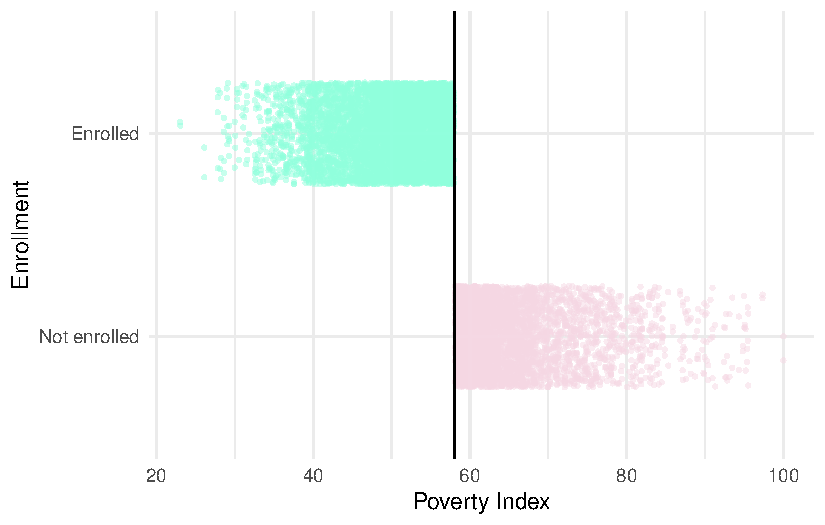
\includegraphics{Jamie-Esmond_problem-set-8_files/figure-pdf/fig-rdd1-1.pdf}

}

\end{figure}

\begin{itemize}
\tightlist
\item
  Determine if the distribution of the running variable
  (\texttt{poverty\_index}) has a jump near the cutoff (it shouldn't).
  (Hint: create a histogram with \texttt{poverty\_index} on the x-axis
  and a vertical line at 58. Use a McCrary test to see if there's a
  significant break in the distribution at 58.)
\end{itemize}

\begin{Shaded}
\begin{Highlighting}[numbers=left,,]
\NormalTok{treat2 }\SpecialCharTok{\%\textgreater{}\%} 
  \FunctionTok{ggplot}\NormalTok{(}\FunctionTok{aes}\NormalTok{(poverty\_index, }\AttributeTok{fill =}\NormalTok{ enrolled)) }\SpecialCharTok{+}
    \FunctionTok{geom\_histogram}\NormalTok{(}\AttributeTok{binwidth =} \DecValTok{2}\NormalTok{, }\AttributeTok{color =} \StringTok{"white"}\NormalTok{, }\AttributeTok{boundary =} \DecValTok{0}\NormalTok{) }\SpecialCharTok{+}
    \FunctionTok{geom\_vline}\NormalTok{(}\AttributeTok{xintercept =} \DecValTok{58}\NormalTok{) }\SpecialCharTok{+}
    \FunctionTok{scale\_fill\_manual}\NormalTok{(}\AttributeTok{values =} \FunctionTok{c}\NormalTok{(}\StringTok{"\#F5D7E3"}\NormalTok{,}\StringTok{"\#90FFDC"}\NormalTok{)) }\SpecialCharTok{+}
    \FunctionTok{labs}\NormalTok{(}\AttributeTok{x =} \StringTok{"Poverty Index"}\NormalTok{,}
         \AttributeTok{y =} \StringTok{"Enrollment"}\NormalTok{,}
         \AttributeTok{fill =} \ConstantTok{NULL}\NormalTok{) }\SpecialCharTok{+}
    \FunctionTok{theme\_minimal}\NormalTok{() }\SpecialCharTok{+} 
    \FunctionTok{theme}\NormalTok{(}\AttributeTok{legend.position =} \StringTok{"bottom"}\NormalTok{)}
\end{Highlighting}
\end{Shaded}

\begin{figure}[H]

\caption{\label{fig-rdd2}RDD - Distribution}

{\centering 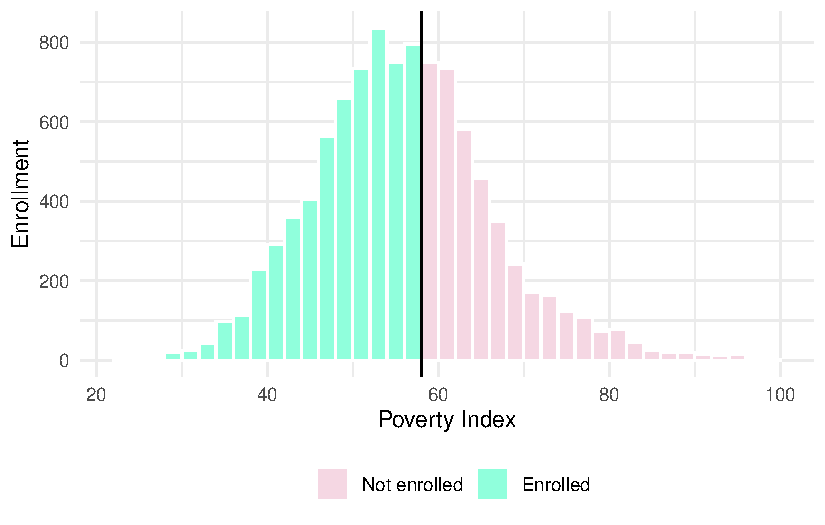
\includegraphics{Jamie-Esmond_problem-set-8_files/figure-pdf/fig-rdd2-1.pdf}

}

\end{figure}

\begin{itemize}
\tightlist
\item
  Visualize the jump in outcome at the cutoff with a scatterplot (Hint:
  create a scatterplot with \texttt{poverty\_index} on the x-axis,
  \texttt{health\_expenditures} on the y-xis, color by
  \texttt{enrolled}, add a vertical line at 58, and add trendlines with
  \texttt{geom\_smooth(method\ =\ "lm")}. You might want to adjust the
  size and transparency of the points with
  \texttt{geom\_point(alpha\ =\ 0.2,\ size\ =\ 0.2)} or something
  similar.)
\end{itemize}

\begin{Shaded}
\begin{Highlighting}[numbers=left,,]
\NormalTok{treat2 }\SpecialCharTok{\%\textgreater{}\%} 
  \FunctionTok{ggplot}\NormalTok{(}\FunctionTok{aes}\NormalTok{(poverty\_index, health\_expenditures, }\AttributeTok{color =}\NormalTok{ enrolled, }\AttributeTok{fill =}\NormalTok{ enrolled)) }\SpecialCharTok{+}
    \FunctionTok{geom\_point}\NormalTok{(}\AttributeTok{alpha =} \FloatTok{0.25}\NormalTok{, }\AttributeTok{pch =} \DecValTok{21}\NormalTok{, }\AttributeTok{size =}\NormalTok{ .}\DecValTok{5}\NormalTok{) }\SpecialCharTok{+}
    \FunctionTok{geom\_smooth}\NormalTok{(}\AttributeTok{method =} \StringTok{"lm"}\NormalTok{, }\AttributeTok{linewidth =} \DecValTok{1}\NormalTok{) }\SpecialCharTok{+}
    \FunctionTok{scale\_color\_manual}\NormalTok{(}\AttributeTok{values =} \FunctionTok{c}\NormalTok{(}\StringTok{"\#F78FB8"}\NormalTok{,}\StringTok{"\#72CCB0"}\NormalTok{)) }\SpecialCharTok{+}
    \FunctionTok{scale\_fill\_manual}\NormalTok{(}\AttributeTok{values =} \FunctionTok{c}\NormalTok{(}\StringTok{"\#F5D7E3"}\NormalTok{,}\StringTok{"\#90FFDC"}\NormalTok{)) }\SpecialCharTok{+}
    \FunctionTok{geom\_vline}\NormalTok{(}\AttributeTok{xintercept =} \DecValTok{58}\NormalTok{) }\SpecialCharTok{+}
    \FunctionTok{labs}\NormalTok{(}\AttributeTok{x =} \StringTok{"Poverty Index"}\NormalTok{,}
         \AttributeTok{y =} \StringTok{"Health Expenditures"}\NormalTok{,}
         \AttributeTok{color =} \ConstantTok{NULL}\NormalTok{,}
         \AttributeTok{fill =} \ConstantTok{NULL}\NormalTok{) }\SpecialCharTok{+}
    \FunctionTok{theme\_minimal}\NormalTok{() }\SpecialCharTok{+} 
    \FunctionTok{theme}\NormalTok{(}\AttributeTok{legend.position =} \StringTok{"bottom"}\NormalTok{)}
\end{Highlighting}
\end{Shaded}

\begin{figure}[H]

\caption{\label{fig-rdd3}RDD - Discontinuity}

{\centering 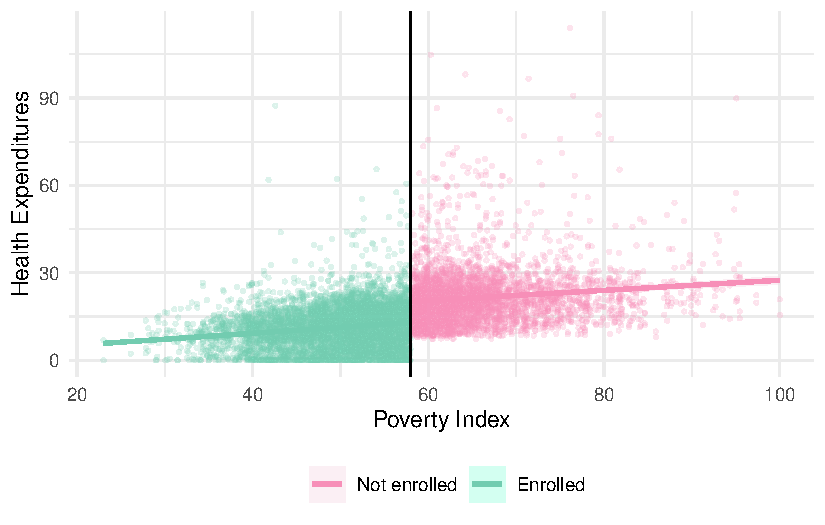
\includegraphics{Jamie-Esmond_problem-set-8_files/figure-pdf/fig-rdd3-1.pdf}

}

\end{figure}

\begin{itemize}
\item
  Graphically, does it look like the HISP reduces health expenditures?

  \begin{itemize}
  \tightlist
  \item
    \textbf{Yes}
  \end{itemize}
\item
  Build a parametric regression model to estimate the size of the gap at
  the cutoff. You'll want to use the centered policy index variable to
  make it easier to interpret. You probably want to create a new dataset
  that only includes observations within some bandwidth that you choose
  (\texttt{filter(poverty\_index\_centered\ \textgreater{}=\ SOMETHING\ \&\ poverty\_index\_centered\ \textless{}=\ SOMETHING)}).
  How big is the effect?
\end{itemize}

\begin{Shaded}
\begin{Highlighting}[numbers=left,,]
\NormalTok{model\_simple }\OtherTok{\textless{}{-}} \FunctionTok{lm}\NormalTok{(health\_expenditures }\SpecialCharTok{\textasciitilde{}}\NormalTok{ poverty\_centered }\SpecialCharTok{+}\NormalTok{ enrolled,}
                   \AttributeTok{data =}\NormalTok{ treat2)}
\FunctionTok{tidy}\NormalTok{(model\_simple)}
\end{Highlighting}
\end{Shaded}

\begin{verbatim}
# A tibble: 3 x 5
  term             estimate std.error statistic   p.value
  <chr>               <dbl>     <dbl>     <dbl>     <dbl>
1 (Intercept)        20.0      0.165      122.  0        
2 poverty_centered    0.190    0.0126      15.0 1.74e- 50
3 enrolledEnrolled   -7.23     0.269      -26.9 9.24e-154
\end{verbatim}

\begin{Shaded}
\begin{Highlighting}[numbers=left,,]
\NormalTok{treat10 }\OtherTok{\textless{}{-}}\NormalTok{ treat2 }\SpecialCharTok{\%\textgreater{}\%} 
  \FunctionTok{filter}\NormalTok{(poverty\_centered }\SpecialCharTok{\textgreater{}=} \SpecialCharTok{{-}}\DecValTok{10} \SpecialCharTok{\&}\NormalTok{ poverty\_centered }\SpecialCharTok{\textless{}=} \DecValTok{10}\NormalTok{)}
\NormalTok{treat5 }\OtherTok{\textless{}{-}}\NormalTok{ treat2 }\SpecialCharTok{\%\textgreater{}\%} 
  \FunctionTok{filter}\NormalTok{(poverty\_centered }\SpecialCharTok{\textgreater{}=} \SpecialCharTok{{-}}\DecValTok{5} \SpecialCharTok{\&}\NormalTok{ poverty\_centered }\SpecialCharTok{\textless{}=} \DecValTok{5}\NormalTok{)}

\NormalTok{model\_simple10 }\OtherTok{\textless{}{-}} \FunctionTok{lm}\NormalTok{(health\_expenditures }\SpecialCharTok{\textasciitilde{}}\NormalTok{ poverty\_centered }\SpecialCharTok{+}\NormalTok{ enrolled,}
                   \AttributeTok{data =}\NormalTok{ treat10)}
\FunctionTok{tidy}\NormalTok{(model\_simple10)}
\end{Highlighting}
\end{Shaded}

\begin{verbatim}
# A tibble: 3 x 5
  term             estimate std.error statistic  p.value
  <chr>               <dbl>     <dbl>     <dbl>    <dbl>
1 (Intercept)        20.0      0.220      90.8  0       
2 poverty_centered    0.236    0.0367      6.45 1.21e-10
3 enrolledEnrolled   -6.82     0.392     -17.4  2.90e-66
\end{verbatim}

\begin{Shaded}
\begin{Highlighting}[numbers=left,,]
\NormalTok{model\_simple5 }\OtherTok{\textless{}{-}} \FunctionTok{lm}\NormalTok{(health\_expenditures }\SpecialCharTok{\textasciitilde{}}\NormalTok{ poverty\_centered }\SpecialCharTok{+}\NormalTok{ enrolled,}
                   \AttributeTok{data =}\NormalTok{ treat5)}
\FunctionTok{tidy}\NormalTok{(model\_simple5)}
\end{Highlighting}
\end{Shaded}

\begin{verbatim}
# A tibble: 3 x 5
  term             estimate std.error statistic  p.value
  <chr>               <dbl>     <dbl>     <dbl>    <dbl>
1 (Intercept)        19.9      0.314      63.4  0       
2 poverty_centered    0.200    0.0975      2.05 4.05e- 2
3 enrolledEnrolled   -7.01     0.560     -12.5  3.05e-35
\end{verbatim}

\begin{itemize}
\tightlist
\item
  Use \texttt{rdrobust()} from the \textbf{rdrobust} library to estimate
  the size of the gap nonparametrically. For the sake of simplicity,
  just use the default (automatic) bandwidth and kernel. How big is the
  effect?
\end{itemize}

\begin{Shaded}
\begin{Highlighting}[numbers=left,,]
\FunctionTok{rdrobust}\NormalTok{(}\AttributeTok{y =}\NormalTok{ treat2}\SpecialCharTok{$}\NormalTok{health\_expenditures, }\AttributeTok{x =}\NormalTok{ treat2}\SpecialCharTok{$}\NormalTok{poverty\_index, }\AttributeTok{c =} \DecValTok{58}\NormalTok{) }\SpecialCharTok{\%\textgreater{}\%}
  \FunctionTok{summary}\NormalTok{()}
\end{Highlighting}
\end{Shaded}

\begin{verbatim}
Sharp RD estimates using local polynomial regression.

Number of Obs.                 9919
BW type                       mserd
Kernel                   Triangular
VCE method                       NN

Number of Obs.                 5929         3990
Eff. Number of Obs.            2498         2130
Order est. (p)                    1            1
Order bias  (q)                   2            2
BW est. (h)                   6.359        6.359
BW bias (b)                  10.803       10.803
rho (h/b)                     0.589        0.589
Unique Obs.                     717          669

=============================================================================
        Method     Coef. Std. Err.         z     P>|z|      [ 95% C.I. ]       
=============================================================================
  Conventional     6.523     0.512    12.729     0.000     [5.519 , 7.528]     
        Robust         -         -    10.590     0.000     [5.236 , 7.614]     
=============================================================================
\end{verbatim}

\newpage

\hypertarget{task-5-ivs2sls}{%
\section{Task 5: IVs/2SLS}\label{task-5-ivs2sls}}

Finally, we can use an instrument to remove the endogeneity from the
choice to enroll in the HISP and estimate the causal effect from
observational data. As you read in chapter 5, World Bank evaluators
randomly selected households to receive encouragement to enroll in HISP.
You can use this encouragement as an instrument for enrollment.

Do the following:

\begin{itemize}
\tightlist
\item
  Create a dataset based on \texttt{hisp} that only includes
  observations from after the intervention (\texttt{round\ ==\ "After"})
\end{itemize}

\begin{Shaded}
\begin{Highlighting}[numbers=left,,]
\NormalTok{after3 }\OtherTok{\textless{}{-}}\NormalTok{ hisp }\SpecialCharTok{\%\textgreater{}\%} 
  \FunctionTok{filter}\NormalTok{(round }\SpecialCharTok{==} \StringTok{"After"}\NormalTok{)}
\end{Highlighting}
\end{Shaded}

\begin{itemize}
\tightlist
\item
  Build a naive regression model that estimates the effect of HISP
  enrollment on health expenditures. You'll need to use the
  \texttt{enrolled\_rp} variable instead of \texttt{enrolled}, since
  we're measuring enrollment after the encouragement intervention.
  (Hint: you'll want to use
  \texttt{health\_expenditures\ \textasciitilde{}\ enrolled\_rp}.) What
  does this naive model tell us about the effect of enrolling in HISP?
\end{itemize}

\begin{Shaded}
\begin{Highlighting}[numbers=left,,]
\NormalTok{model\_naive2 }\OtherTok{\textless{}{-}} \FunctionTok{lm}\NormalTok{(health\_expenditures }\SpecialCharTok{\textasciitilde{}}\NormalTok{ enrolled\_rp,}
                   \AttributeTok{data =}\NormalTok{ after3)}
\FunctionTok{tidy}\NormalTok{(model\_naive2)}
\end{Highlighting}
\end{Shaded}

\begin{verbatim}
# A tibble: 2 x 5
  term        estimate std.error statistic p.value
  <chr>          <dbl>     <dbl>     <dbl>   <dbl>
1 (Intercept)     20.6     0.124     166.        0
2 enrolled_rp    -12.7     0.229     -55.5       0
\end{verbatim}

\begin{itemize}
\tightlist
\item
  Check the relevance, exclusion, and exogeneity of promotion
  (\texttt{promotion\_locality}) as an instrument. For relevance, you'll
  want to run a model that predicts enrollment based on promotion (hint:
  \texttt{enrolled\_rp\ \textasciitilde{}\ promotion\_locality}) and
  check (1) the significance of the coefficient and (2) the F-statistic.
  For exclusion and exogeneity, you'll have to tell a convincing story
  that proves promotion influences health expenditures \emph{only
  through} HISP enrollment.
\end{itemize}

\begin{Shaded}
\begin{Highlighting}[numbers=left,,]
\NormalTok{model\_promo }\OtherTok{\textless{}{-}} \FunctionTok{lm}\NormalTok{(enrolled\_rp }\SpecialCharTok{\textasciitilde{}}\NormalTok{ promotion\_locality,}
                   \AttributeTok{data =}\NormalTok{ after3)}
\FunctionTok{tidy}\NormalTok{(model\_promo)}
\end{Highlighting}
\end{Shaded}

\begin{verbatim}
# A tibble: 2 x 5
  term                        estimate std.error statistic  p.value
  <chr>                          <dbl>     <dbl>     <dbl>    <dbl>
1 (Intercept)                   0.0842   0.00586      14.4 1.97e-46
2 promotion_localityPromotion   0.408    0.00818      49.8 0       
\end{verbatim}

\begin{Shaded}
\begin{Highlighting}[numbers=left,,]
\FunctionTok{glance}\NormalTok{(model\_promo)}
\end{Highlighting}
\end{Shaded}

\begin{verbatim}
# A tibble: 1 x 12
  r.squared adj.r.squ~1 sigma stati~2 p.value    df logLik    AIC    BIC devia~3
      <dbl>       <dbl> <dbl>   <dbl>   <dbl> <dbl>  <dbl>  <dbl>  <dbl>   <dbl>
1     0.200       0.200 0.407   2485.       0     1 -5158. 10322. 10343.   1643.
# ... with 2 more variables: df.residual <int>, nobs <int>, and abbreviated
#   variable names 1: adj.r.squared, 2: statistic, 3: deviance
\end{verbatim}

\begin{itemize}
\tightlist
\item
  Run a 2SLS regression model with promotion as the instrument. You can
  do this by hand if you want (i.e.~run a first stage model, extract
  predicted enrollment, and use predicted enrollment as the second
  stage), \emph{or} you can just use the \texttt{iv\_robust()} function
  from the \textbf{estimatr} library. (Hint: you'll want to use
  \texttt{health\_expenditures\ \textasciitilde{}\ enrolled\_rp\ \textbar{}\ promotion\_locality}
  as the formula). After removing the endogeneity from enrollment, what
  is the casual effect of enrollment in the HISP on health expenditures?
\end{itemize}

\begin{Shaded}
\begin{Highlighting}[numbers=left,,]
\NormalTok{model\_iv }\OtherTok{\textless{}{-}} \FunctionTok{iv\_robust}\NormalTok{(health\_expenditures }\SpecialCharTok{\textasciitilde{}}\NormalTok{ enrolled\_rp }\SpecialCharTok{|}\NormalTok{ promotion\_locality,}
          \AttributeTok{data =}\NormalTok{ after3, }\AttributeTok{diagnostics =} \ConstantTok{TRUE}\NormalTok{)}
\FunctionTok{summary}\NormalTok{(model\_iv)}
\end{Highlighting}
\end{Shaded}

\begin{verbatim}

Call:
iv_robust(formula = health_expenditures ~ enrolled_rp | promotion_locality, 
    data = after3, diagnostics = TRUE)

Standard error type:  HC2 

Coefficients:
            Estimate Std. Error t value Pr(>|t|) CI Lower CI Upper   DF
(Intercept)     19.6      0.181   108.8 0.00e+00     19.3    20.00 9912
enrolled_rp     -9.5      0.516   -18.4 2.29e-74    -10.5    -8.49 9912

Multiple R-squared:  0.222 ,    Adjusted R-squared:  0.222 
F-statistic:  339 on 1 and 9912 DF,  p-value: <2e-16

Diagnostics:
                 numdf dendf  value p.value    
Weak instruments     1  9912 2552.2  <2e-16 ***
Wu-Hausman           1  9911   43.7   4e-11 ***
Overidentifying      0    NA     NA      NA    
---
Signif. codes:  0 '***' 0.001 '**' 0.01 '*' 0.05 '.' 0.1 ' ' 1
\end{verbatim}

\begin{itemize}
\tightlist
\item
  Show the results from the two regressions in a side-by-side table if
  you want
\end{itemize}

\begin{Shaded}
\begin{Highlighting}[numbers=left,,]
\NormalTok{together5 }\OtherTok{\textless{}{-}} \FunctionTok{modelsummary}\NormalTok{(}\FunctionTok{list}\NormalTok{(}\StringTok{"Naive"} \OtherTok{=}\NormalTok{ model\_naive2,}
                               \StringTok{"2SLS"} \OtherTok{=}\NormalTok{ model\_iv),}
             \AttributeTok{coef\_rename =} \FunctionTok{c}\NormalTok{(}\AttributeTok{enrolled\_rp =} \StringTok{"Enrolled"}\NormalTok{),}
             \AttributeTok{output =} \StringTok{"kableExtra"}\NormalTok{,}
             \AttributeTok{estimate =} \StringTok{"\{estimate\}\{stars\}"}\NormalTok{,}
             \AttributeTok{statistic =} \StringTok{"statistic"}\NormalTok{,}
             \AttributeTok{fmt =}  \DecValTok{3}\NormalTok{,}
             \AttributeTok{gof\_omit =} \StringTok{"IC|Log|Adj|p}\SpecialCharTok{\textbackslash{}\textbackslash{}}\StringTok{.value|statistic|se\_type|F|RMSE"}\NormalTok{) }\SpecialCharTok{\%\textgreater{}\%} 
  \FunctionTok{row\_spec}\NormalTok{(}\FunctionTok{c}\NormalTok{(}\DecValTok{1}\NormalTok{,}\DecValTok{3}\NormalTok{), }\AttributeTok{background =} \StringTok{"\#8DE4FF"}\NormalTok{) }

\NormalTok{together5}
\end{Highlighting}
\end{Shaded}

\hypertarget{tbl-iv}{}
\begin{table}
\caption{\label{tbl-iv}IV/2SLS }\tabularnewline

\centering
\begin{tabular}[t]{lcc}
\toprule
  & Naive & 2SLS\\
\midrule
\cellcolor[HTML]{8DE4FF}{(Intercept)} & \cellcolor[HTML]{8DE4FF}{\num{20.587}***} & \cellcolor[HTML]{8DE4FF}{\num{19.646}***}\\
 & (\num{165.879}) & (\num{108.752})\\
\cellcolor[HTML]{8DE4FF}{Enrolled} & \cellcolor[HTML]{8DE4FF}{\num{-12.708}***} & \cellcolor[HTML]{8DE4FF}{\num{-9.500}***}\\
 & (\num{-55.458}) & (\num{-18.399})\\
\midrule
Num.Obs. & \num{9914} & \num{9914}\\
R2 & \num{0.237} & \num{0.222}\\
\bottomrule
\end{tabular}
\end{table}

\newpage

\hypertarget{task-6-summary}{%
\section{Task 6: Summary}\label{task-6-summary}}

You just calculated a bunch of causal effects. List them here. Which one
do you trust the most? Why?

\textbf{RCT is the most trustworthy, of course, because it's most
similar to an experiment, but since RCTs are not always possible or
ethical, the diff-in-diff or 2SLS are the causal effects that I would
trust the most in this situation.}

\textbf{Diff-in-diff uses the logic that the locations offered treatment
and the the locations that were not offered treatment are not
fundamentally different. Therefore, by comparing the change in the
treatment locations and the control locations, the causal effect is the
difference between the changes in each location. Normally, we would want
to confirm that the trends for the outcome were parallel before
treatment, to support the argument that without treatment the trends
would have continued to be parallel.}

\textbf{The 2SLS model assumes that the households who randomly selected
for promotion of the treatment are not fundamentally different from
those who did not receive the promotion. Since the promotion of the
program is correlated with enrollment, enrollment is correlated with
lower health expenditures, promotion meets the relevancy requirement as
an instrument. It is also obvious that promotion is not going to
influence health expenditures through any path besides enrollment.
Lastly, promotion is exogenous because households selected for promotion
were selected randomly. By removing the endogeneity from enrollment
through promotion, a trustworthy causal effect can be estimated. (Also,
I know that there is about a ten point effect in this data and 2SLS
model is the closest and has the best story.)}

\begin{Shaded}
\begin{Highlighting}[numbers=left,,]
\NormalTok{alltogethernow }\OtherTok{\textless{}{-}} \FunctionTok{modelsummary}\NormalTok{(}\FunctionTok{list}\NormalTok{(}\StringTok{"Naive"} \OtherTok{=}\NormalTok{ model\_naive,}
                                    \StringTok{"RCT"} \OtherTok{=}\NormalTok{ he\_after,}
                                    \StringTok{"IPW"} \OtherTok{=}\NormalTok{ model\_ipw,}
                                    \StringTok{"Matching"} \OtherTok{=}\NormalTok{ model\_matched,}
                                    \StringTok{"Diff{-}in{-}Diff"} \OtherTok{=}\NormalTok{ model\_diff,}
                                    \StringTok{"RDD (BW 10)"} \OtherTok{=}\NormalTok{ model\_simple10,}
                                    \StringTok{"2SLS"} \OtherTok{=}\NormalTok{ model\_iv),}
             \AttributeTok{coef\_rename =} \FunctionTok{c}\NormalTok{(}\AttributeTok{enrolledEnrolled =} \StringTok{"Enrolled"}\NormalTok{,}
                             \AttributeTok{treatment\_localityTreatment =} \StringTok{"Treatment"}\NormalTok{,}
                             \AttributeTok{roundAfter =} \StringTok{"After"}\NormalTok{,}
                             \AttributeTok{poverty\_centered =} \StringTok{"Poverty Level"}\NormalTok{,}
                             \AttributeTok{enrolled\_rp =} \StringTok{"Enrolled"}\NormalTok{),}
             \AttributeTok{output =} \StringTok{"kableExtra"}\NormalTok{,}
             \AttributeTok{estimate =} \StringTok{"\{estimate\}\{stars\}"}\NormalTok{,}
             \AttributeTok{statistic =} \StringTok{"statistic"}\NormalTok{,}
             \AttributeTok{fmt =}  \DecValTok{2}\NormalTok{,}
             \AttributeTok{gof\_omit =} \StringTok{"IC|Log|Adj|p}\SpecialCharTok{\textbackslash{}\textbackslash{}}\StringTok{.value|statistic|se\_type|F|RMSE"}\NormalTok{) }\SpecialCharTok{\%\textgreater{}\%} 
  \FunctionTok{row\_spec}\NormalTok{(}\FunctionTok{c}\NormalTok{(}\DecValTok{1}\NormalTok{,}\DecValTok{3}\NormalTok{,}\DecValTok{5}\NormalTok{,}\DecValTok{7}\NormalTok{,}\DecValTok{9}\NormalTok{,}\DecValTok{11}\NormalTok{), }\AttributeTok{background =} \StringTok{"\#8DE4FF"}\NormalTok{) }\SpecialCharTok{\%\textgreater{}\%} 
  \FunctionTok{column\_spec}\NormalTok{(}\DecValTok{1}\NormalTok{, }\AttributeTok{width =} \StringTok{"5.5em"}\NormalTok{) }\SpecialCharTok{\%\textgreater{}\%} 
  \FunctionTok{column\_spec}\NormalTok{(}\DecValTok{2}\SpecialCharTok{:}\DecValTok{8}\NormalTok{, }\AttributeTok{width =} \StringTok{"4em"}\NormalTok{)}


\NormalTok{alltogethernow }\SpecialCharTok{\%\textgreater{}\%} 
  \FunctionTok{kable\_styling}\NormalTok{(}\AttributeTok{font\_size =} \FloatTok{9.5}\NormalTok{)}
\end{Highlighting}
\end{Shaded}

\hypertarget{tbl-alltogethernow}{}
\begin{table}
\caption{\label{tbl-alltogethernow}All Together Now! }\tabularnewline

\centering
\fontsize{9.5}{11.5}\selectfont
\begin{tabular}[t]{>{\raggedright\arraybackslash}p{5.5em}>{\centering\arraybackslash}p{4em}>{\centering\arraybackslash}p{4em}>{\centering\arraybackslash}p{4em}>{\centering\arraybackslash}p{4em}>{\centering\arraybackslash}p{4em}>{\centering\arraybackslash}p{4em}>{\centering\arraybackslash}p{4em}}
\toprule
  & Naive & RCT & IPW & Matching & Diff-in-Diff & RDD (BW 10) & 2SLS\\
\midrule
\cellcolor[HTML]{8DE4FF}{(Intercept)} & \cellcolor[HTML]{8DE4FF}{\num{20.71}***} & \cellcolor[HTML]{8DE4FF}{\num{20.06}***} & \cellcolor[HTML]{8DE4FF}{\num{19.46}***} & \cellcolor[HTML]{8DE4FF}{\num{17.90}***} & \cellcolor[HTML]{8DE4FF}{\num{20.79}***} & \cellcolor[HTML]{8DE4FF}{\num{19.98}***} & \cellcolor[HTML]{8DE4FF}{\num{19.65}***}\\
 & (\num{167.13}) & (\num{123.32}) & (\num{155.43}) & (\num{94.06}) & (\num{117.36}) & (\num{90.81}) & (\num{108.75})\\
\cellcolor[HTML]{8DE4FF}{Enrolled} & \cellcolor[HTML]{8DE4FF}{\num{-12.87}***} & \cellcolor[HTML]{8DE4FF}{} & \cellcolor[HTML]{8DE4FF}{\num{-11.06}***} & \cellcolor[HTML]{8DE4FF}{\num{-10.06}***} & \cellcolor[HTML]{8DE4FF}{\num{-6.30}***} & \cellcolor[HTML]{8DE4FF}{\num{-6.82}***} & \cellcolor[HTML]{8DE4FF}{\num{-9.50}***}\\
 & (\num{-56.79}) &  & (\num{-57.11}) & (\num{-41.90}) & (\num{-27.50}) & (\num{-17.39}) & (\num{-18.40})\\
\cellcolor[HTML]{8DE4FF}{Treatment} & \cellcolor[HTML]{8DE4FF}{} & \cellcolor[HTML]{8DE4FF}{\num{-6.41}***} & \cellcolor[HTML]{8DE4FF}{} & \cellcolor[HTML]{8DE4FF}{} & \cellcolor[HTML]{8DE4FF}{} & \cellcolor[HTML]{8DE4FF}{} & \cellcolor[HTML]{8DE4FF}{}\\
 &  & (\num{-27.85}) &  &  &  &  & \\
\cellcolor[HTML]{8DE4FF}{After} & \cellcolor[HTML]{8DE4FF}{} & \cellcolor[HTML]{8DE4FF}{} & \cellcolor[HTML]{8DE4FF}{} & \cellcolor[HTML]{8DE4FF}{} & \cellcolor[HTML]{8DE4FF}{\num{1.51}***} & \cellcolor[HTML]{8DE4FF}{} & \cellcolor[HTML]{8DE4FF}{}\\
 &  &  &  &  & (\num{6.04}) &  & \\
\cellcolor[HTML]{8DE4FF}{Enrolled:After} & \cellcolor[HTML]{8DE4FF}{} & \cellcolor[HTML]{8DE4FF}{} & \cellcolor[HTML]{8DE4FF}{} & \cellcolor[HTML]{8DE4FF}{} & \cellcolor[HTML]{8DE4FF}{\num{-8.16}***} & \cellcolor[HTML]{8DE4FF}{} & \cellcolor[HTML]{8DE4FF}{}\\
 &  &  &  &  & (\num{-25.19}) &  & \\
\cellcolor[HTML]{8DE4FF}{Poverty Level} & \cellcolor[HTML]{8DE4FF}{} & \cellcolor[HTML]{8DE4FF}{} & \cellcolor[HTML]{8DE4FF}{} & \cellcolor[HTML]{8DE4FF}{} & \cellcolor[HTML]{8DE4FF}{} & \cellcolor[HTML]{8DE4FF}{\num{0.24}***} & \cellcolor[HTML]{8DE4FF}{}\\
 &  &  &  &  &  & (\num{6.45}) & \\
\midrule
Num.Obs. & \num{9914} & \num{9914} & \num{9914} & \num{4718} & \num{9919} & \num{6648} & \num{9914}\\
R2 & \num{0.246} & \num{0.073} & \num{0.248} & \num{0.271} & \num{0.344} & \num{0.228} & \num{0.222}\\
\bottomrule
\end{tabular}
\end{table}



\end{document}
